\documentclass[11pt,letterpaper]{article}
\usepackage{fontspec}
\setmainfont{texgyrepagella}[Extension=.otf,UprightFont=*-regular,BoldFont=*-bold,ItalicFont=*-italic,BoldItalicFont=*-bolditalic]
\usepackage[bidi=default]{babel}
\babelprovide[import,main]{spanish}
\babelprovide[import]{hebrew}
\babelprovide[import]{ancientgreek}
\babelfont[hebrew]{rm}[Path=fonts/,BoldFont=NotoHebrewSerif-700.ttf,Scale=0.95]{NotoHebrewSerif-400.ttf}
\babelfont[ancientgreek]{rm}[Path=fonts/]{GFSPorson.otf}
\newcommand{\heb}[1]{\mbox{\foreignlanguage{hebrew}{#1}}}
\newcommand{\grc}[1]{\foreignlanguage{ancientgreek}{#1}}
\newcommand{\hebverso}[1]{\par\smallskip{\centering\begin{otherlanguage}{hebrew}\large #1\end{otherlanguage}\par}\smallskip}
\newcommand{\SENOR}{\textsc{Señor}}
\usepackage[margin=2.5cm,headheight=14pt]{geometry}
\usepackage{microtype,ragged2e,booktabs,graphicx,xcolor,csquotes,array}
\usepackage[hidelinks]{hyperref}\usepackage{xurl}\urlstyle{same}
\usepackage[most]{tcolorbox}
\usepackage{tikz}\usetikzlibrary{arrows.meta,positioning,calc,decorations.pathreplacing}
\usepackage{titlesec,fancyhdr}
\definecolor{azul}{HTML}{15437C}\definecolor{azuloscuro}{HTML}{0B1F3A}\definecolor{celeste}{HTML}{5694D6}
\definecolor{dorado}{RGB}{196,154,60}\definecolor{papiro}{RGB}{246,239,220}\definecolor{gris}{RGB}{70,78,96}
\titleformat{\section}{\Large\bfseries\color{azul}}{\thesection.}{0.6em}{}
\titleformat{\subsection}{\large\bfseries\color{azuloscuro}}{\thesubsection}{0.6em}{}
\pagestyle{fancy}\fancyhf{}
\fancyhead[L]{\foreignlanguage{spanish}{\small\itshape\color{gris}Dios es Espíritu}}\fancyhead[R]{\foreignlanguage{spanish}{\small\color{gris}\thepage}}
\renewcommand{\headrulewidth}{0.4pt}
\setlength{\parindent}{1.27cm}\linespread{1.15}\setlength{\emergencystretch}{3em}
\newtcolorbox{cita}[1][]{enhanced,colback=azul!6!white,colframe=azul,boxrule=0pt,leftrule=2.5pt,arc=0pt,
  left=8pt,right=8pt,top=5pt,bottom=5pt,before skip=8pt,after skip=8pt,fontupper=\itshape,#1}
\newcommand{\fuente}[1]{\par\hfill{\upshape\bfseries\small\textcolor{azul}{#1}}}
\newtcolorbox{nota}[1][]{enhanced,colback=dorado!10,colframe=dorado!85!azul,boxrule=0.6pt,arc=2pt,
  fonttitle=\bfseries\small,coltitle=azuloscuro,colbacktitle=dorado!30,fontupper=\small,title={#1}}
\newtcolorbox{filologia}[1][]{enhanced,colback=white,colframe=azul!45,boxrule=0.5pt,arc=2pt,
  fonttitle=\bfseries\small,coltitle=white,colbacktitle=azul!80,fontupper=\small,title={Filología: #1}}
\newcommand{\refapa}[1]{\par{\RaggedRight\hangindent=1.27cm\hangafter=1\noindent #1\par}\vspace{4pt}}
\newcommand{\destacar}[1]{\textbf{\textcolor{azul}{#1}}}
\newcolumntype{L}[1]{>{\RaggedRight\arraybackslash}p{#1}}


\title{\color{azul}\bfseries Dios es Espíritu\\[4pt]\large\color{gris}\mdseries ``Dios es Espíritu; y los que le adoran, en espíritu y en verdad es necesario que adoren'' (Jn 4:24)}
\author{}\date{}
\begin{document}
\maketitle\thispagestyle{empty}

\begin{abstract}\noindent
La definición más breve que la Biblia da de Dios cabe en tres palabras griegas, \grc{πνεῦμα ὁ θεός}, ``Dios es Espíritu'' (Jn 4:24), y Jesús la pronunció junto al pozo de Jacob, ante una mujer samaritana que le preguntaba por lugares de culto. Este capítulo parte de ese texto (Jn 4:19--24) y estudia la palabra hebrea \emph{rúaj}, que reúne viento, aliento y espíritu, junto con su equivalente griego \emph{pneûma} y el espectro completo de ambas en la Reina-Valera 1960. Presenta el título que revela el atributo, ``Dios de los espíritus de toda carne'' (Nm 16:22; 27:16), y lo define: Dios existe sin cuerpo, sin partes y sin forma visible, es vida en sí mismo y fuente de toda vida, y se da a conocer por su palabra y en el Hijo. Aclara después lo que el atributo no significa y cómo han de leerse las imágenes corporales de la Escritura, y expone su teología desde los textos: un Dios sin cuerpo y por eso presente en todo lugar, invisible pero revelado, vivo y dador de vida. El encuentro en la historia de Israel es Horeb, donde Dios habló ``de en medio del fuego'' y el pueblo oyó una voz, ``mas a excepción de oír la voz, ninguna figura'' vio (Dt 4:12). El capítulo recoge luego la mirada del judaísmo (el alma y el Santo en \emph{Berajot} 10a; Maimónides y el \emph{Yigdal}; los targumes; Qumrán) y lee el atributo en Cristo con Pablo: la imagen del Dios invisible (Col 1:15), ``el Señor es el Espíritu'' (2 Co 3:17), el templo que es un pueblo (Ef 2:22) y el postrer Adán, ``espíritu vivificante'' (1 Co 15:45). Termina preguntando qué significa adorar a un Dios que es Espíritu.
\par\smallskip\noindent\textbf{Palabras clave:} espíritu, \emph{rúaj}, \emph{pneûma}, incorporeidad, invisibilidad, adoración, imagen, Horeb, Sicar.\end{abstract}

\begin{nota}[Nota sobre el texto]
Las citas bíblicas son de la Reina-Valera 1960. Donde esta escribe ``Jehová'', aquí se escribe \SENOR, que traduce el tetragrama \heb{יהוה}, leído en la tradición judía como \emph{Adonay}. El hebreo sigue la BHS; el griego, NA28 y la Septuaginta de Rahlfs-Hanhart. Las fuentes judías (Talmud, Targum, Rashi, Maimónides, liturgia) se citan desde Sefaria, y los textos de Qumrán desde las ediciones de García Martínez (1992) y Vermes (2004); todo lo que es interpretación se marca como precisión. Cuando la numeración hebrea difiere de la española se da entre corchetes.
\end{nota}

%===================================================================
\section{Tres palabras en un pozo}

Es mediodía en Samaria. Jesús, ``cansado del camino'', se ha sentado junto al pozo de Jacob cuando una mujer llega a sacar agua (Jn 4:6--7). La conversación empieza por el agua y desemboca en una de las frases más densas de toda la Escritura:

\begin{cita}Dios es Espíritu; y los que le adoran, en espíritu y en verdad es necesario que adoren.\fuente{(Jn 4:24)}\end{cita}

En griego son tres palabras, \grc{πνεῦμα ὁ θεός}, ``espíritu (es) Dios''. No es una definición dictada en una escuela de filosofía, sino la respuesta a una pregunta sobre dónde se debe adorar. La mujer pregunta por un \destacar{lugar}, Gerizim o Jerusalén, y Jesús responde con el \destacar{ser} de Dios: porque Dios es Espíritu, el lugar deja de ser la pregunta. El atributo no aparece aquí como especulación, sino como la razón de una adoración nueva.

Esta serie agrupa en el Ser lo que responde a la pregunta ``¿qué es Dios?''. Juan ofrece tres fórmulas con la misma forma: ``Dios es Espíritu'' (Jn 4:24), ``Dios es luz'' (1 Jn 1:5) y ``Dios es amor'' (1 Jn 4:8). Pink las reúne como las ``tres cosas que nos dicen las Escrituras con respecto a la naturaleza de Dios'' (Pink, 2020, cap. 16, p. 83).

\begin{center}
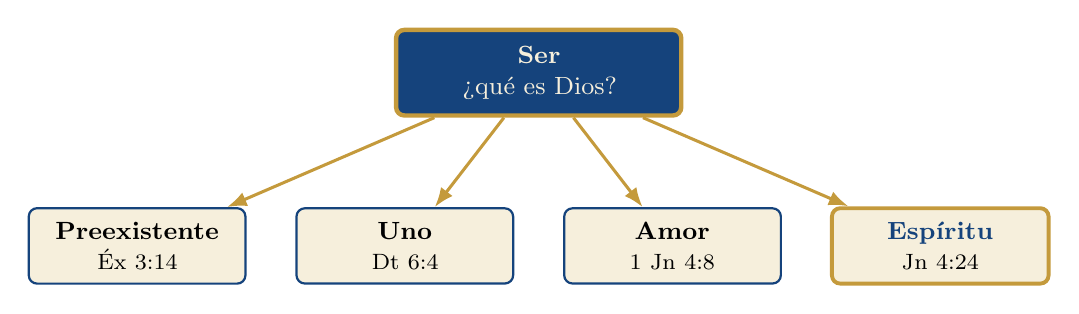
\begin{tikzpicture}[font=\small,
  caja/.style={draw=azul,line width=0.8pt,fill=papiro,rounded corners=3pt,inner sep=5pt,align=center}]
 \node[draw=dorado,line width=1.6pt,fill=azul,text=papiro,rounded corners=3pt,text width=3.2cm,align=center,inner sep=6pt] (s) at (0,1.9) {\textbf{Ser}\\ ¿qué es Dios?};
 \node[caja,text width=2.4cm] (p) at (-5.1,-0.3) {\textbf{Preexistente}\\ {\footnotesize Éx 3:14}};
 \node[caja,text width=2.4cm] (u) at (-1.7,-0.3) {\textbf{Uno}\\ {\footnotesize Dt 6:4}};
 \node[caja,text width=2.4cm] (a) at (1.7,-0.3) {\textbf{Amor}\\ {\footnotesize 1 Jn 4:8}};
 \node[draw=dorado,line width=1.4pt,fill=papiro,rounded corners=3pt,text width=2.4cm,align=center,inner sep=5pt] (e) at (5.1,-0.3) {\textbf{\textcolor{azul}{Espíritu}}\\ {\footnotesize Jn 4:24}};
 \foreach \i in {p,u,a,e}\draw[-{Latex[length=2.5mm]},dorado,line width=1.1pt](s)--(\i);
\end{tikzpicture}\par
{\footnotesize\color{gris}\textit{Figura 1.} El atributo dentro de la Parte I (Ser). \textit{Nota.} Elaboración propia según la clasificación de la serie.}
\end{center}

\begin{nota}[Precisión]
Clasificación propuesta: atributo del Ser; \emph{incomunicable} en su esencia, porque Dios es espíritu increado, infinito y fuente de todo espíritu; \emph{comunicable} como reflejo, porque Dios ``forma el espíritu del hombre dentro de él'' (Zac 12:1).
\end{nota}

``Espíritu'' es una de las palabras más frecuentes de la Biblia. Un conteo propio sobre la RVR1960, sin títulos de sección y con los números Strong, arroja estas cifras:

\begin{center}\small\renewcommand{\arraystretch}{1.18}
\begin{tabular}{@{}L{4.2cm}L{5.4cm}r@{}}
\toprule
\textbf{Forma (RVR1960)} & \textbf{Original más frecuente} & \textbf{Veces} \\ \midrule
espíritu & \heb{רוּחַ} \emph{rúaj}, \grc{πνεῦμα} \emph{pneûma} & 608 \\
espíritus & \heb{רוּחוֹת}, \grc{πνεύματα} & 36 \\
espiritual & \grc{πνευματικός} & 19 \\
espirituales & \grc{πνευματικός} & 10 \\
espiritualmente & \grc{πνευματικῶς} & 1 \\ \midrule
\textbf{Total} & \textbf{607 versículos (262 AT, 412 NT)} & \textbf{674} \\
\bottomrule
\end{tabular}\par
{\footnotesize\color{gris}\textit{Tabla 1.} ``Espíritu'' y sus formas en la RVR1960. \textit{Nota.} Conteo propio con la RVR1960 sin títulos de sección; los versículos del AT y del NT suman más de 607 porque se cuentan las apariciones por testamento. Verificar en e-Sword.}
\end{center}

El verso que vertebra esta obra pide gloriarse en ``entenderme y conocerme'' (Jer 9:24 [9:23]). Saber que Dios es Espíritu es saber, antes que nada, que no se le conoce como se conoce una cosa: no se le ve, no se le toca, no se le encierra. Y, con todo, se le conoce, porque él habla y se acerca.

%===================================================================
\section{Texto ancla: Juan 4:19--24}

\subsection{Sicar, el pozo de Jacob}

\begin{cita}Vino, pues, a una ciudad de Samaria llamada Sicar, junto a la heredad que Jacob dio a su hijo José. Y estaba allí el pozo de Jacob.\fuente{(Jn 4:5--6)}\end{cita}

El diálogo ocurre en tierra de patriarcas. Allí levantó Abram su primer altar en Canaán, en ``el lugar de Siquem'' (Gn 12:6--7); allí compró Jacob un campo y erigió un altar al que llamó ``El-Elohe-Israel'' (Gn 33:18--20); y frente a Siquem se alza Gerizim, el monte de la bendición (Dt 11:29; 27:12). Tras la caída de Samaria, los colonos traídos por Asiria ``temían a \SENOR, y honraban a sus dioses'' (2 R 17:24, 33). Cuando la mujer pregunta, pregunta con siglos de historia a la espalda.

\begin{center}
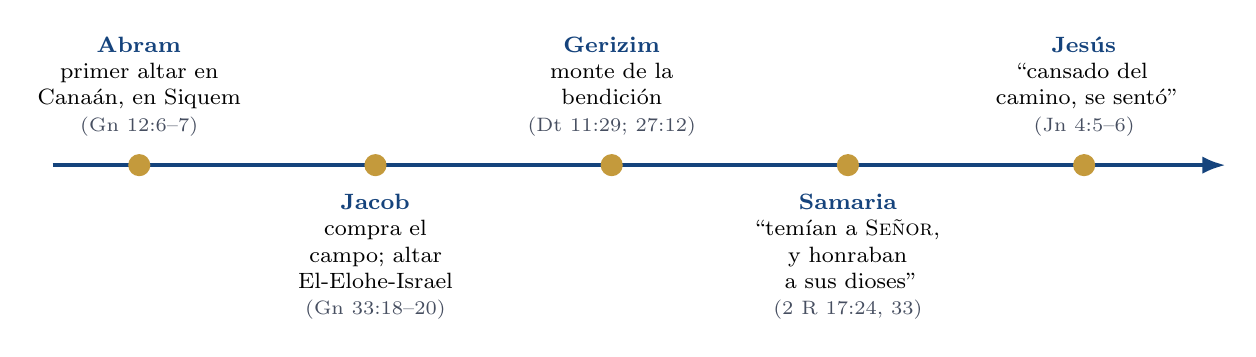
\begin{tikzpicture}[font=\footnotesize]
 \draw[line width=1.6pt,azul,-{Latex[length=3mm]}] (-0.3,0) -- (14.6,0);
 \foreach \x/\t/\b/\r/\pos in {0.8/{Abram}/{primer altar en Canaán, en Siquem}/{Gn 12:6--7}/above,
   3.8/{Jacob}/{compra el campo; altar El-Elohe-Israel}/{Gn 33:18--20}/below,
   6.8/{Gerizim}/{monte de la bendición}/{Dt 11:29; 27:12}/above,
   9.8/{Samaria}/{``temían a \SENOR, y honraban a sus dioses''}/{2 R 17:24, 33}/below,
   12.8/{Jesús}/{``cansado del camino, se sentó''}/{Jn 4:5--6}/above}{
  \fill[dorado] (\x,0) circle (4pt);
  \node[\pos=7pt,text width=2.6cm,align=center] at (\x,0) {\textbf{\textcolor{azul}{\t}}\\ \b\\ {\scriptsize\color{gris}(\r)}};}
\end{tikzpicture}\par
{\footnotesize\color{gris}\textit{Figura 2.} Siquem y Gerizim en la historia bíblica. \textit{Nota.} Elaboración propia.}
\end{center}

\subsection{``¿Este monte o Jerusalén?''}

\begin{cita}Le dijo la mujer: Señor, me parece que tú eres profeta. Nuestros padres adoraron en este monte, y vosotros decís que en Jerusalén es el lugar donde se debe adorar.\fuente{(Jn 4:19--20)}\end{cita}

Samaritanos y judíos compartían la Torá, pero no el lugar del culto. La disputa se apoyaba en textos y arrastraba una historia de violencia:

\begin{center}\small\renewcommand{\arraystretch}{1.22}
\begin{tabular}{@{}L{2.2cm}L{6.0cm}L{6.0cm}@{}}
\toprule
 & \textbf{Samaritanos: Gerizim} & \textbf{Judíos: Jerusalén} \\ \midrule
Canon & solo el Pentateuco & Ley, Profetas y Escritos \\
Base & altares de Abram y Jacob en Siquem (Gn 12:6--7; 33:20); la bendición en Gerizim (Dt 11:29; 27:12) & ``el lugar que \SENOR{} vuestro Dios escogiere'' (Dt 12:5), identificado con Sion (2 Cr 6:6; Sal 132:13) \\
Texto & el Pentateuco samaritano lee ``Gerizim'' en Dt 27:4 (TM: ``Ebal'') y añade Gerizim al Decálogo & el TM lee ``Ebal'' en Dt 27:4 \\
Templo & construido en Gerizim; destruido por Juan Hircano (129 a.\,e.\,c.) & segundo templo, en pie en tiempos de Jesús \\
\bottomrule
\end{tabular}\par
{\footnotesize\color{gris}\textit{Tabla 2.} La disputa sobre el lugar de culto. \textit{Nota.} Elaboración propia a partir de Tov (2012), la \emph{Encyclopaedia Judaica} (2007, ``Gerizim, Mount'') y MacArthur (2011, nota a Jn 4:20).}
\end{center}

\begin{nota}[Precisión textual]
Las lecturas del Pentateuco samaritano siguen a Tov (2012). La \emph{Encyclopaedia Judaica} (2007) fecha la destrucción del templo de Gerizim en 129 a.\,e.\,c., según Josefo (\emph{Antigüedades} 13.255--256).
\end{nota}

\subsection{El texto}

\begin{cita}Jesús le dijo: Mujer, créeme, que la hora viene cuando ni en este monte ni en Jerusalén adoraréis al Padre. Vosotros adoráis lo que no sabéis; nosotros adoramos lo que sabemos; porque la salvación viene de los judíos. Mas la hora viene, y ahora es, cuando los verdaderos adoradores adorarán al Padre en espíritu y en verdad; porque también el Padre tales adoradores busca que le adoren. Dios es Espíritu; y los que le adoran, en espíritu y en verdad es necesario que adoren.\fuente{(Jn 4:21--24)}\end{cita}

\begin{filologia}[Jn 4:23--24]
\begin{tabular}{@{}L{3.6cm}L{1.6cm}L{9.6cm}@{}}
\grc{ἔρχεται ὥρα καὶ νῦν ἐστιν} & \grc{ἔρχομαι} & ``viene la hora, y ahora es'': lo futuro ya empezó con Jesús (cf. Jn 5:25). \\[2pt]
\grc{προσκυνέω} \emph{proskynéō} & \grc{κυνέω} & ``adorar'', postrarse; 9 veces en 4:20--24. La LXX lo usa para \heb{הִשְׁתַּחֲוָה} \emph{hishtajavá}, ``inclinarse'' (Éx 20:5). \\[2pt]
\grc{πνεῦμα ὁ θεός} & \grc{πνέω} & ``Espíritu (es) Dios'': el predicado va primero y sin artículo; describe qué es Dios, no lo pone en una clase (``un espíritu''). \\[2pt]
\grc{ἐν πνεύματι καὶ ἀληθείᾳ} & --- & una sola preposición para los dos sustantivos: una sola manera de adorar. \\[2pt]
\grc{δεῖ} \emph{deî} & --- & ``es necesario'': el mismo verbo de la mujer en 4:20 (``donde se debe adorar''). Jesús cambia el dónde por el cómo. \\
\end{tabular}
\end{filologia}

Pink repara en el mismo detalle gramatical: ``En el griego, no hay un artículo indefinido y decir `Dios es un espíritu' es muy objetable, puesto que lo ubica en una clase con otros. Dios es `espíritu' en el sentido más elevado'' (Pink, 2020, cap. 16, p. 83).

\subsection{Del lugar a la manera}

El argumento de Jesús avanza en cuatro pasos. La mujer pregunta \emph{dónde} (4:20); Jesús anuncia una \emph{hora} en que ni este monte ni Jerusalén serán el centro (4:21); afirma a continuación la \emph{historia} de la revelación, porque ``la salvación viene de los judíos'' (4:22); y lo funda todo, por último, en el \emph{ser} de Dios (4:24).

\begin{center}
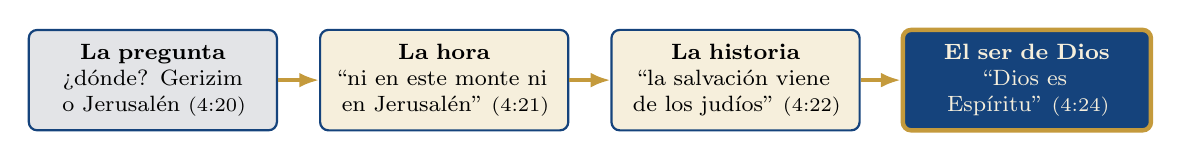
\begin{tikzpicture}[font=\footnotesize,
  caja/.style={draw=azul,line width=0.8pt,fill=papiro,rounded corners=3pt,inner sep=5pt,align=center,text width=2.8cm}]
 \node[caja,fill=gris!15] (a) at (0,0) {\textbf{La pregunta}\\ ¿dónde? Gerizim o Jerusalén {\scriptsize(4:20)}};
 \node[caja] (b) at (3.7,0) {\textbf{La hora}\\ ``ni en este monte ni en Jerusalén'' {\scriptsize(4:21)}};
 \node[caja] (c) at (7.4,0) {\textbf{La historia}\\ ``la salvación viene de los judíos'' {\scriptsize(4:22)}};
 \node[draw=dorado,line width=1.6pt,fill=azul,text=papiro,rounded corners=3pt,text width=2.8cm,align=center,inner sep=5pt] (d) at (11.1,0) {\textbf{El ser de Dios}\\ ``Dios es Espíritu'' {\scriptsize(4:24)}};
 \draw[-{Latex[length=2.5mm]},dorado,line width=1.2pt] (a)--(b); \draw[-{Latex[length=2.5mm]},dorado,line width=1.2pt] (b)--(c); \draw[-{Latex[length=2.5mm]},dorado,line width=1.2pt] (c)--(d);
\end{tikzpicture}\par
{\footnotesize\color{gris}\textit{Figura 3.} El argumento de Jn 4:20--24. \textit{Nota.} Elaboración propia.}
\end{center}

Jesús no relativiza la revelación: ``nosotros adoramos lo que sabemos''. La salvación tiene historia y tiene pueblo. Pero el Dios de esa historia no está atado a un monte, y lo que antes se ligaba a un lugar se liga ahora a una persona y a una manera. La iniciativa, además, es de Dios: el Padre ``busca'' (\grc{ζητεῖ}) adoradores. Salomón ya lo había reconocido al dedicar el templo:

\begin{cita}Pero ¿es verdad que Dios morará sobre la tierra? He aquí que los cielos, los cielos de los cielos, no te pueden contener; ¿cuánto menos esta casa que yo he edificado?\fuente{(1 R 8:27)}\end{cita}

\subsection{``En espíritu y en verdad''}

La expresión admite dos lecturas principales, que la tabla resume:

\begin{center}\small\renewcommand{\arraystretch}{1.22}
\begin{tabular}{@{}L{3.0cm}L{5.6cm}L{5.6cm}@{}}
\toprule
\textbf{Lectura} & \textbf{Sentido} & \textbf{Apoyo} \\ \midrule
Espíritu humano & adorar desde lo interior, no solo con ritos y lugares & MacArthur (2011, nota a Jn 4:24); Is 66:2, ``humilde de espíritu'' \\
Espíritu Santo & adorar movidos por el Espíritu que Jesús dará & Jn 3:5--6; 7:38--39: el agua viva ``dijo del Espíritu'' \\
``Verdad'' & conforme a la revelación, centrada en Jesús & Jn 1:14, 17; 14:6 \\
\bottomrule
\end{tabular}\par
{\footnotesize\color{gris}\textit{Tabla 3.} Lecturas de ``en espíritu y en verdad''. \textit{Nota.} Elaboración propia.}
\end{center}

En ese mismo capítulo, Jesús había ofrecido a la mujer un agua distinta:

\begin{cita}mas el que bebiere del agua que yo le daré, no tendrá sed jamás; sino que el agua que yo le daré será en él una fuente de agua que salte para vida eterna.\fuente{(Jn 4:14)}\end{cita}

Más adelante el evangelista explica qué era esa agua: ``Esto dijo del Espíritu que habían de recibir los que creyesen en él'' (Jn 7:39). La adoración ``en espíritu'' corresponde, así, a lo que Dios \destacar{es}: el adorador ha de ser semejante al adorado. Por eso el agua viva (4:14) y la adoración nueva (4:24) van juntas.

\begin{nota}[Precisión]
La referencia de ``espíritu'' en Jn 4:23--24 (espíritu humano o Espíritu Santo) se discute. El contexto de Juan, donde el agua viva es el Espíritu (7:39), favorece que el espíritu humano adore movido por el Espíritu de Dios. Es una lectura propia de esta serie.
\end{nota}

%===================================================================
\section{La palabra: \emph{rúaj}, viento, aliento, espíritu}

\subsection{Una palabra con cuatro rostros}

El hebreo carece de una palabra para ``inmaterial''. Para decir lo que Dios es recurre a una palabra concreta, \heb{רוּחַ} \emph{rúaj}, que nombra a la vez el viento, el aliento y el espíritu. Lo que sus sentidos tienen en común es algo \destacar{real, invisible y poderoso}: el viento no se ve, pero se ven sus efectos; el aliento no se ve, pero se ve la vida.

\begin{center}
\begin{tikzpicture}[font=\footnotesize,
  caja/.style={draw=azul,line width=0.8pt,fill=papiro,rounded corners=3pt,inner sep=5pt,align=center,text width=3.6cm}]
 \node[draw=dorado,line width=1.6pt,fill=azul,text=papiro,circle,minimum size=2cm,align=center] (c) at (0,0) {\heb{רוּחַ}\\ \emph{rúaj}};
 \node[caja] (v) at (-4.6,1.3) {\textbf{Viento}\\ ``por recio viento oriental'' {\scriptsize(Éx 14:21)}};
 \node[caja] (a) at (4.6,1.3) {\textbf{Aliento}\\ ``por el aliento de su boca'' {\scriptsize(Sal 33:6)}};
 \node[caja] (h) at (-4.6,-1.4) {\textbf{Vida, ánimo}\\ ``el espíritu vuelva a Dios que lo dio'' {\scriptsize(Ec 12:7)}};
 \node[caja] (e) at (4.6,-1.4) {\textbf{Espíritu de Dios}\\ ``el Espíritu de Dios se movía'' {\scriptsize(Gn 1:2)}};
 \foreach \i in {v,a,h,e}\draw[dorado,line width=1.1pt] (c)--(\i);
\end{tikzpicture}\par
{\footnotesize\color{gris}\textit{Figura 4.} Los sentidos de \emph{rúaj}. \textit{Nota.} Elaboración propia a partir de Vine (1999) y Chávez (1992).}
\end{center}

Vine (1999) agrupa los usos en aliento, aire fugaz, viento, ánimo y espíritu; Chávez (1992) distingue entre ellos el ``espíritu, distinto e independiente del factor material'' (Pr 16:2; Is 31:3).

\subsection{Génesis 1:2 y 2:7: el Espíritu que se cierne y el aliento que da vida}

\hebverso{וְרוּחַ אֱלֹהִים מְרַחֶפֶת עַל־פְּנֵי הַמָּיִם}
\begin{cita}Y la tierra estaba desordenada y vacía, y las tinieblas estaban sobre la faz del abismo, y el Espíritu de Dios se movía sobre la faz de las aguas.\fuente{(Gn 1:2)}\end{cita}

\begin{filologia}[Gn 1:2]
\begin{tabular}{@{}L{3.2cm}L{1.6cm}L{10cm}@{}}
\heb{רוּחַ אֱלֹהִים} \emph{rúaj Elohim} & \heb{רוח} & ``Espíritu de Dios''. Es la primera aparición de \emph{rúaj} en la Biblia: el Espíritu de Dios presente en la creación. \\[2pt]
\heb{מְרַחֶפֶת} \emph{merajéfet} & \heb{רחף} & ``se cernía'', ``revoloteaba''. El mismo verbo describe al águila que ``revolotea sobre sus pollos'' (\heb{יְרַחֵף}, Dt 32:11). \\
\end{tabular}
\end{filologia}

\begin{nota}[Precisión]
La lectura de Gn 1:2 como ``viento de Dios'' es antigua. El Targum Ónkelos traduce \heb{וְרוּחָא מִן קֳדָם יְיָ מְנַשְּׁבָא}, ``y un viento de delante del \SENOR{} soplaba''. La RVR1960 lee ``Espíritu''.
\end{nota}

\hebverso{וַיִּפַּח בְּאַפָּיו נִשְׁמַת חַיִּים}
\begin{cita}Entonces \SENOR{} Dios formó al hombre del polvo de la tierra, y sopló en su nariz aliento de vida, y fue el hombre un ser viviente.\fuente{(Gn 2:7)}\end{cita}

\begin{filologia}[Gn 2:7]
\begin{tabular}{@{}L{3.2cm}L{1.6cm}L{10cm}@{}}
\heb{וַיִּפַּח} \emph{vayyipaj} & \heb{נפח} & ``y sopló'': el hombre vive porque Dios sopla. \\[2pt]
\heb{נִשְׁמַת חַיִּים} \emph{nishmat jayyim} & \heb{נשׁם} & ``aliento de vida''. \emph{Neshamá} es ``aliento, hálito''; la RVR1960 la traduce ``espíritu'' en Job 26:4 y Pr 20:27: ``Lámpara de \SENOR{} es el espíritu del hombre''. \\
\end{tabular}
\end{filologia}

Un mismo vocabulario sirve para la creación del cosmos y para la del hombre: ``Por la palabra de \SENOR{} fueron hechos los cielos, y todo el ejército de ellos por el aliento de su boca'' (Sal 33:6, \heb{וּבְרוּחַ פִּיו}). Lo que Dios dice y lo que Dios sopla dan, a la vez, existencia y vida.

\subsection{El espectro completo}

La tabla reúne el espectro completo: los términos hebreos, arameos y griegos que la RVR1960 traduce con ``espíritu'', junto con las palabras emparentadas.

\begin{center}\small\renewcommand{\arraystretch}{1.18}
\begin{tabular}{@{}L{3.3cm}L{3.3cm}L{4.0cm}L{3.6cm}@{}}
\toprule
\textbf{Término} & \textbf{Sentido} & \textbf{RVR1960} & \textbf{Textos} \\ \midrule
\heb{רוּחַ} \emph{rúaj} (H7307) & viento, aliento, ánimo, espíritu & espíritu ($\approx$\,200), viento(s) ($\approx$\,74), aliento, soplo, hálito, aire, lado & Gn 1:2; 8:1; Nm 16:22; Is 31:3; Ez 37:9 \\
\heb{רוּחַ} \emph{rúaj} (arameo, H7308) & viento; espíritu, mente & espíritu, viento & Dn 2:35; 4:8; 5:12; 7:15 \\
\heb{נְשָׁמָה} \emph{neshamá} (H5397) & soplo, aliento vital & aliento, espíritu, soplo & Gn 2:7; Job 26:4; Pr 20:27 \\
\heb{נֶפֶשׁ} \emph{néfesh} & aliento, vida, persona & ``amargura de espíritu'' (\heb{מַר־נֶפֶשׁ}) & 1 S 22:2 \\ \midrule
\grc{πνεῦμα} \emph{pneûma} (379) & viento, aliento, espíritu, Espíritu & espíritu, viento, aliento & Jn 3:8; 4:24; Ro 8:16; 2 Ts 2:8 \\
\grc{πνευματικός} (26) & espiritual & espiritual(es) & Ro 7:14; 1 Co 2:13--15; 15:44 \\
\grc{πνευματικῶς} (2) & espiritualmente & espiritualmente, en sentido espiritual & 1 Co 2:14; Ap 11:8 \\
\grc{πνοή} (2) & soplo, aliento & viento, aliento & Hch 2:2; 17:25 \\
\grc{πνέω} (7) & soplar & soplar & Jn 3:8; Hch 27:40 \\
\grc{ἐκπνέω} (3) & expirar & expirar & Mr 15:37; Lc 23:46 \\
\grc{θεόπνευστος} (1) & ``soplada por Dios'' & inspirada por Dios & 2 Ti 3:16 \\
\bottomrule
\end{tabular}\par
{\footnotesize\color{gris}\textit{Tabla 4.} Espectro hebreo, arameo y griego de ``espíritu''. \textit{Nota.} Conteo propio con la BHS y la NA27 (números Strong) y la RVR1960; los conteos por traducción son aproximados. Verificar en e-Sword.}
\end{center}

El conteo propio en la BHS da para \emph{rúaj} 376 apariciones en 349 versículos (366 en hebreo y 10 en arameo), con el etiquetado Strong incompleto; Vine (1999) habla de ``unas 378'' para el hebreo. Los libros donde más aparece son Ezequiel (51) e Isaías (49). Conviene no confundirla con \heb{רָוַח} (1 S 16:23, ``tenía alivio''), de la misma raíz \emph{r-w-ḥ}, ``respirar, tener holgura''.

La Septuaginta traduce \emph{rúaj} casi siempre con \grc{πνεῦμα}, y el griego conserva el doble sentido. Jesús juega con él ante Nicodemo:

\begin{cita}El viento sopla de donde quiere, y oyes su sonido; mas ni sabes de dónde viene, ni a dónde va; así es todo aquel que es nacido del Espíritu.\fuente{(Jn 3:8)}\end{cita}

``El viento'' es \grc{τὸ πνεῦμα}; ``del Espíritu'' es \grc{ἐκ τοῦ πνεύματος}. Una misma palabra dice las dos cosas.

\begin{nota}[Precisión]
\grc{φάντασμα} (``fantasma'', Mt 14:26; Mr 6:49) no se traduce ``espíritu''. En Lc 24:37 la RVR1960 traduce \grc{πνεῦμα} ``espíritu''.
\end{nota}

\subsection{``Carne, y no espíritu''}

El texto del Antiguo Testamento que más se acerca a Jn 4:24 no está en un salmo, sino en una advertencia política. Judá buscaba ayuda militar en Egipto y confiaba en sus carros y en sus caballos (Is 31:1). Isaías responde:

\hebverso{וּמִצְרַיִם אָדָם וְלֹא־אֵל \\ וְסוּסֵיהֶם בָּשָׂר וְלֹא־רוּחַ}
\begin{cita}Y los egipcios hombres son, y no Dios; y sus caballos carne, y no espíritu; de manera que al extender \SENOR{} su mano, caerá el ayudador y caerá el ayudado, y todos ellos desfallecerán a una.\fuente{(Is 31:3)}\end{cita}

El paralelismo es exacto: hombre // carne; Dios // espíritu. Isaías opone la \destacar{carne} perecedera al \destacar{espíritu} que pertenece a Dios, y con ello invierte el cálculo de Judá: lo que se ve y se cuenta, caballos, carros y ejércitos, es lo débil; lo que no se ve es lo fuerte.

\begin{center}
\begin{tikzpicture}[font=\small,
  caja/.style={draw=azul,line width=0.8pt,fill=gris!15,rounded corners=3pt,inner sep=5pt,align=center,text width=2.6cm},
  dios/.style={draw=dorado,line width=1.4pt,fill=azul,text=papiro,rounded corners=3pt,inner sep=5pt,align=center,text width=2.6cm}]
 \node[caja] (a) at (0,1.2) {\heb{אָדָם} hombre};
 \node[dios] (b) at (5,1.2) {\heb{אֵל} Dios};
 \node[caja] (c) at (0,0) {\heb{בָּשָׂר} carne};
 \node[dios] (d) at (5,0) {\heb{רוּחַ} espíritu};
 \draw[<->,gris,thick] (a)--(b) node[midway,above,font=\footnotesize]{no es};
 \draw[<->,gris,thick] (c)--(d) node[midway,above,font=\footnotesize]{no es};
\end{tikzpicture}\par
{\footnotesize\color{gris}\textit{Figura 5.} El paralelismo de Is 31:3. \textit{Nota.} Elaboración propia.}
\end{center}

\begin{nota}[Precisión textual]
La LXX no tiene ``y no espíritu'': lee \grc{καὶ οὐκ ἔστιν βοήθεια}, ``y no hay ayuda''. El Targum conserva \heb{בְּסַר וְלָא רוּחַ}.
\end{nota}

\subsection{Los ídolos: forma sin espíritu}

Si Dios es espíritu sin forma, el ídolo es exactamente lo contrario: forma sin espíritu.

\begin{cita}Todo hombre se embrutece, y le falta ciencia; se avergüenza de su ídolo todo fundidor, porque mentirosa es su obra de fundición, y no hay espíritu en ella.\fuente{(Jer 10:14)}\end{cita}

\begin{cita}¡Ay del que dice al palo: Despiértate; y a la piedra muda: Levántate! ¿Podrá él enseñar? He aquí está cubierto de oro y plata, y no hay espíritu dentro de él.\fuente{(Hab 2:19)}\end{cita}

En hebreo, \heb{וְלֹא־רוּחַ בָּם} (Jer 10:14) y \heb{וְכָל־רוּחַ אֵין בְּקִרְבּוֹ} (Hab 2:19). El Salmo lo dice del aliento: ``Tampoco hay aliento en sus bocas'' (Sal 135:17, \heb{רוּחַ}). El ídolo tiene boca y no respira; el Dios verdadero no tiene forma visible y es todo vida.

\begin{nota}[Precisión]
Jer 10:14 pertenece al texto ancla del atributo Verdadero (Jer 10:1--16): allí el ídolo es mentira porque no tiene espíritu.
\end{nota}

%===================================================================
\section{El Nombre que revela su ser espiritual}

\subsection{``Dios de los espíritus de toda carne''}

El Antiguo Testamento no conoce un nombre propio ``Espíritu'' para Dios. Conoce, en cambio, un título que aparece dos veces en Números, siempre en boca de Moisés y siempre en oración:

\hebverso{אֵל אֱלֹהֵי הָרוּחֹת לְכָל־בָּשָׂר}
\begin{cita}Y ellos se postraron sobre sus rostros, y dijeron: Dios, Dios de los espíritus de toda carne, ¿no es un solo hombre el que pecó? ¿Por qué airarte contra toda la congregación?\fuente{(Nm 16:22)}\end{cita}

\begin{cita}Ponga \SENOR, Dios de los espíritus de toda carne, un varón sobre la congregación.\fuente{(Nm 27:16)}\end{cita}

\begin{filologia}[Nm 16:22]
\begin{tabular}{@{}L{3.6cm}L{1.6cm}L{9.6cm}@{}}
\heb{אֵל אֱלֹהֵי} & \heb{אל} & ``Dios, Dios de\ldots'': vocativo doble en la oración de Moisés y Aarón. \\[2pt]
\heb{הָרוּחֹת} \emph{harujot} & \heb{רוח} & ``los espíritus'', plural de \emph{rúaj}: el aliento vital de cada ser humano. \\[2pt]
\heb{לְכָל־בָּשָׂר} & \heb{בשׂר} & ``de toda carne'': toda criatura viviente. \\[2pt]
LXX & --- & \grc{θεὸς θεὸς τῶν πνευμάτων καὶ πάσης σαρκός}: ``Dios de los espíritus y de toda carne''. \\[2pt]
Ónkelos & --- & \heb{אֵל אֱלָהּ רוּחַיָּא לְכָל בִּשְׂרָא}: conserva la fórmula. \\
\end{tabular}
\end{filologia}

Las dos veces la fórmula surge en una situación límite. En Nm 16, tras la rebelión de Coré, Moisés apela al Dios que conoce cada espíritu para que no castigue a toda la congregación por el pecado de unos pocos; en Nm 27, al acercarse su muerte, pide a ese mismo Dios un sucesor, y recibe a Josué. El título sostiene las dos súplicas: el Dios de los espíritus juzga con justicia porque conoce el interior de cada uno, y provee pastores porque sabe lo que cada uno necesita.

Rashi lo entendió así en ambos textos:

\begin{quote}\itshape
``Conoce los pensamientos'' (\heb{יוֹדֵעַ מַחֲשָׁבוֹת}). Un rey de carne y sangre, si una provincia peca contra él, no sabe quién pecó y castiga a todos; ``pero tú, ante ti están revelados todos los pensamientos''.\par\hfill{\upshape\small\bfseries\textcolor{azul}{(Rashi a Nm 16:22)}}
\end{quote}

\begin{quote}\itshape
``Manifiesto ante ti es el pensamiento de cada uno, y no se parecen entre sí''; pon sobre ellos un guía que soporte a cada uno según su manera de pensar.\par\hfill{\upshape\small\bfseries\textcolor{azul}{(Rashi a Nm 27:16)}}
\end{quote}

\begin{nota}[Precisión]
Comentario rabínico medieval (Sefaria); traducción propia.
\end{nota}

\subsection{El que forma y da el espíritu}

Los profetas desarrollan el título en forma de participios. Dios es ``el que da aliento al pueblo que mora sobre ella, y espíritu a los que por ella andan'' (Is 42:5), y es también el que ``forma el espíritu del hombre dentro de él'':

\begin{cita}Profecía de la palabra de \SENOR{} acerca de Israel. \SENOR, que extiende los cielos y funda la tierra, y forma el espíritu del hombre dentro de él, ha dicho:\fuente{(Zac 12:1)}\end{cita}

El Nuevo Testamento recoge la misma fórmula: ``¿Por qué no obedeceremos mucho mejor al Padre de los espíritus, y viviremos?'' (He 12:9).

\begin{center}\small\renewcommand{\arraystretch}{1.22}
\begin{tabular}{@{}L{4.3cm}L{4.6cm}L{2.0cm}L{3.4cm}@{}}
\toprule
\textbf{Nombre o título} & \textbf{Hebreo / griego} & \textbf{Texto} & \textbf{Qué revela} \\ \midrule
Dios de los espíritus de toda carne & \heb{אֱלֹהֵי הָרוּחֹת לְכָל־בָּשָׂר} & Nm 16:22; 27:16 & dueño y conocedor de todo espíritu \\
El que forma el espíritu del hombre & \heb{יֹצֵר רוּחַ־אָדָם} & Zac 12:1 & fuente del espíritu humano \\
El que da aliento y espíritu & \heb{נֹתֵן נְשָׁמָה}\ldots{} \heb{וְרוּחַ} & Is 42:5 & dador de la vida \\
Padre de los espíritus & \grc{τῷ πατρὶ τῶν πνευμάτων} & He 12:9 & relación paternal \\
Dios de los espíritus de los profetas & \grc{ὁ θεὸς τῶν πνευμάτων τῶν προφητῶν} & Ap 22:6 & el que habla por los profetas \\
El Invisible & \grc{τὸν ἀόρατον} & He 11:27 & no se le ve, pero sostiene \\
\bottomrule
\end{tabular}\par
{\footnotesize\color{gris}\textit{Tabla 5.} Los nombres y títulos que revelan que Dios es Espíritu. \textit{Nota.} Elaboración propia.}
\end{center}

\begin{nota}[Precisión]
No hay un nombre propio ``Espíritu'' en el Antiguo Testamento. Se usa el título ``Dios de los espíritus'', que lo revela como fuente y dueño de todo espíritu. El Nombre que revela el atributo es, en esta serie, Nm 16:22, como se anunció en el mapa de los nombres de la Introducción.
\end{nota}

%===================================================================
\section{Definición}

\begin{tcolorbox}[colback=papiro,colframe=azul,boxrule=1pt,arc=3pt,title={Definición},colbacktitle=azul,coltitle=papiro]
Que Dios es Espíritu es la perfección eterna de su ser por la cual Dios existe sin cuerpo, sin partes y sin forma visible; es vida en sí mismo y fuente de toda vida; no está limitado por lugar ni puede ser representado por imagen; y se da a conocer por su palabra, por su Espíritu y, en plenitud, en el Hijo hecho carne.
\end{tcolorbox}

\begin{nota}[Precisión]
Definición de síntesis de esta serie, a partir de los textos estudiados.
\end{nota}

La definición reúne seis rasgos, y cada uno tiene su base en un texto concreto:

\begin{center}\small\renewcommand{\arraystretch}{1.22}
\begin{tabular}{@{}L{3.6cm}L{10.6cm}@{}}
\toprule
\textbf{Rasgo} & \textbf{Texto} \\ \midrule
Incorpóreo & ``un espíritu no tiene carne ni huesos, como veis que yo tengo'' (Lc 24:39) \\
Invisible & ``al Rey de los siglos, inmortal, invisible, al único y sabio Dios'' (1 Ti 1:17) \\
Vivo y vivificante & ``El espíritu es el que da vida; la carne para nada aprovecha'' (Jn 6:63) \\
Sin límite de lugar & ``¿A dónde me iré de tu Espíritu?'' (Sal 139:7) \\
Sin imagen & ``ninguna figura visteis el día que \SENOR{} habló con vosotros'' (Dt 4:15) \\
Personal & ``el Padre tales adoradores busca que le adoren'' (Jn 4:23) \\
\bottomrule
\end{tabular}\par
{\footnotesize\color{gris}\textit{Tabla 6.} Los rasgos del atributo. \textit{Nota.} Elaboración propia.}
\end{center}

\subsection{Lo que no significa}

Decir que Dios es Espíritu se presta a malentendidos. La tabla recoge cinco de los más frecuentes y lo que la Escritura responde a cada uno:

\begin{center}\small\renewcommand{\arraystretch}{1.25}
\begin{tabular}{@{}L{4.0cm}L{10.2cm}@{}}
\toprule
\textbf{Malentendido} & \textbf{Respuesta bíblica} \\ \midrule
``Un espíritu entre otros'' & Es ``Padre de los espíritus'' (He 12:9); los demás espíritus son criaturas (Zac 12:1). \\
Fuerza impersonal, energía & Habla, busca, ama: ``el Padre tales adoradores busca'' (Jn 4:23). \\
Irreal, vago, lejano & Es lo más real: ``las cosas que se ven son temporales, pero las que no se ven son eternas'' (2 Co 4:18). \\
Hostil a lo material & Creó la materia y la llamó ``bueno en gran manera'' (Gn 1:31); en Cristo habita ``corporalmente'' (Col 2:9). \\
Solo ``el Espíritu Santo'' & ``Dios es Espíritu'' describe el ser mismo de Dios, el Padre a quien se adora (Jn 4:23--24); no es solo un nombre del Espíritu Santo. \\
\bottomrule
\end{tabular}\par
{\footnotesize\color{gris}\textit{Tabla 7.} Malentendidos sobre el atributo. \textit{Nota.} Elaboración propia.}
\end{center}

\subsection{Manos, ojos, alas: el lenguaje de los hombres}

La Biblia habla de Dios con imágenes tomadas del cuerpo: ``al extender \SENOR{} su mano'' (Is 31:3); ``los ojos de \SENOR{} contemplan toda la tierra'' (2 Cr 16:9); ``bajo sus alas estarás seguro'' (Sal 91:4); ``El cielo es mi trono'' (Is 66:1). Son \emph{antropomorfismos}, lenguaje humano para hablar del poder, del cuidado y del gobierno de Dios. Esas imágenes son verdaderas \emph{como imágenes}: Dios actúa, ve y protege de veras, pero no tiene miembros. La misma Torá que dice ``mano'' prohíbe hacer una figura de Dios (Dt 4:15--16).

Los sabios condensaron este principio en una frase que Maimónides hizo clásica:

\hebverso{דִּבְּרָה תוֹרָה כִּלְשׁוֹן בְּנֵי אָדָם}
\begin{quote}\itshape
``La Torá habló en el lenguaje de los hombres''.\par\hfill{\upshape\small\bfseries\textcolor{azul}{(Berajot 31b, citado por Maimónides, Yesodé haTorá 1:9)}}
\end{quote}

\begin{nota}[Precisión]
El principio rabínico se cita según Maimónides, \emph{Mishné Torá}, Yesodé haTorá 1:9, y su comentario a la Misná, Sanedrín 10:1 (Sefaria).
\end{nota}

%===================================================================
\section{Teología: el Dios que es Espíritu}

\subsection{Incorpóreo, y por eso presente en todo lugar}

Decir que Dios es Espíritu es decir, ante todo, que no tiene cuerpo. Y lo que no tiene cuerpo no cabe encerrado en un lugar: no se lo puede situar en Gerizim ni en Jerusalén, ni dejarlo atrás al cambiar de tierra. La primera consecuencia teológica del atributo es, por eso, una presencia sin límites. Así lo razona Pink al comentar Jn 4:24:

\begin{quote}\itshape
Debido a que es ``espíritu'', es incorpóreo, no tiene sustancia visible. Si Dios tuviera un cuerpo tangible, no sería omnipresente, estaría limitado a un lugar; pero precisamente porque es ``espíritu'', llena el cielo y la tierra.\par\hfill{\upshape\small\bfseries\textcolor{azul}{(Pink, 2020, cap. 16, p. 83)}}
\end{quote}

La Escritura lo había dicho mucho antes, en forma de oración y con el paralelismo propio de la poesía hebrea:

\hebverso{אָנָה אֵלֵךְ מֵרוּחֶךָ וְאָנָה מִפָּנֶיךָ אֶבְרָח}
\begin{cita}¿A dónde me iré de tu Espíritu? ¿Y a dónde huiré de tu presencia? Si subiere a los cielos, allí estás tú; Y si en el Seol hiciere mi estrado, he aquí, allí tú estás.\fuente{(Sal 139:7--8)}\end{cita}

``Tu Espíritu'' // ``tu presencia'' (\heb{פָּנֶיךָ}, literalmente ``tu rostro''). Porque es Espíritu, Dios no ocupa un lugar: está en todo lugar. ``¿No lleno yo, dice \SENOR, el cielo y la tierra?'' (Jer 23:24). Lo que en Jn 4 suprime el monte, en el Salmo 139 suprime la huida. Este rasgo se estudiará por extenso en el atributo \emph{Omnipresente}.

\subsection{Invisible, pero revelado}

\begin{cita}Dijo más: No podrás ver mi rostro; porque no me verá hombre, y vivirá.\fuente{(Éx 33:20)}\end{cita}

\begin{cita}el único que tiene inmortalidad, que habita en luz inaccesible; a quien ninguno de los hombres ha visto ni puede ver, al cual sea la honra y el imperio sempiterno. Amén.\fuente{(1 Ti 6:16)}\end{cita}

Ningún ser humano ``ha visto ni puede ver'' a Dios, y no por distancia, sino por lo que Dios es. La invisibilidad no es un velo que el esfuerzo humano pueda descorrer algún día; pertenece a su ser. De ahí se sigue algo decisivo para la teología: si Dios es Espíritu, no se lo alcanza por los sentidos ni se lo deduce por la sola razón; se lo conoce cuando él mismo se da a conocer. Por eso Israel recibió en Horeb una voz y no una figura, y por eso el Nombre se proclama antes de que el rostro se vea (Éx 34:5--7). Pink, que cita 1 Ti 6:16 al presentar a Dios como ``independiente de todo'', funda la misma conclusión en el texto de Juan:

\begin{quote}\itshape
Tampoco Dios es conocido por el intelecto. Dios es Espíritu (Jn. 4:24) y, por lo tanto, sólo puede ser conocido espiritualmente.\par\hfill{\upshape\small\bfseries\textcolor{azul}{(Pink, 2020, cap. 1, p. 9)}}
\end{quote}

Pablo describe ese conocimiento con las palabras de la creación: ``Porque Dios, que mandó que de las tinieblas resplandeciese la luz, es el que resplandeció en nuestros corazones, para iluminación del conocimiento de la gloria de Dios en la faz de Jesucristo'' (2 Co 4:6). El Dios que dijo ``Sea la luz'' (Gn 1:3) es el que alumbra el corazón; la luz no sube del hombre hacia Dios, baja de Dios al hombre. Pink subraya que ese resplandor ocurre ``en nuestros corazones (y no en nuestros intelectos)'' (Pink, 2020, cap. 1). El Dios invisible no es, entonces, un Dios mudo ni lejano: Moisés no vio su rostro, pero oyó su Nombre (Éx 34:5--7), y la gloria que nadie puede ver se ha dejado ver ``en la faz de Jesucristo''.

\begin{nota}[Precisión]
La autoría paulina de 1 Timoteo se discute; la misma idea aparece en cartas indiscutidas: ``las cosas invisibles de él, su eterno poder y deidad'' (Ro 1:20).
\end{nota}

\subsection{Espíritu que da vida}

\hebverso{מֵאַרְבַּע רוּחוֹת בֹּאִי הָרוּחַ}
\begin{cita}Y me dijo: Profetiza al espíritu, profetiza, hijo de hombre, y dí al espíritu: Así ha dicho \SENOR{} el Señor: Espíritu, ven de los cuatro vientos, y sopla sobre estos muertos, y vivirán.\fuente{(Ez 37:9)}\end{cita}

``De los cuatro \emph{rujot} ven, \emph{rúaj}'': viento, aliento y Espíritu caben en una sola frase. Dios mismo explica después la visión: ``Y pondré mi Espíritu en vosotros, y viviréis'' (Ez 37:14, \heb{רוּחִי}). El Dios que es Espíritu está vivo y da vida, y Jesús lo dirá con palabras muy semejantes: ``El espíritu es el que da vida; la carne para nada aprovecha; las palabras que yo os he hablado son espíritu y son vida'' (Jn 6:63). Los ídolos no tienen \emph{rúaj} (Jer 10:14); el Dios vivo la \emph{da}.

\subsection{Un reflejo en el ser humano}

Dios \destacar{dio} espíritu al ser humano (Gn 2:7; Zac 12:1; Ec 12:7), y por eso el atributo es comunicable como reflejo. Pablo se sirve de esa analogía para hablar del conocimiento de Dios:

\begin{cita}Porque ¿quién de los hombres sabe las cosas del hombre, sino el espíritu del hombre que está en él? Así tampoco nadie conoció las cosas de Dios, sino el Espíritu de Dios.\fuente{(1 Co 2:11)}\end{cita}

Como el espíritu del hombre conoce lo íntimo del hombre, solo el Espíritu de Dios conoce lo íntimo de Dios. La analogía, sin embargo, tiene un límite: el espíritu humano es dado, limitado y unido a un cuerpo, mientras que el de Dios es increado. ``El polvo vuelva a la tierra, como era, y el espíritu vuelva a Dios que lo dio'' (Ec 12:7).

\begin{nota}[Precisión]
1 Co 2:10--11 es el texto que este libro usa como marco de humildad: lo profundo de Dios solo lo conoce su Espíritu, y lo conocemos porque ``Dios nos las reveló a nosotros por el Espíritu'' (1 Co 2:10).
\end{nota}

%===================================================================
\section{Un encuentro en la historia de Israel: Horeb, una voz sin figura}

\subsection{``Ninguna figura visteis''}

Cuarenta años después del Sinaí, en las llanuras de Moab, Moisés recuerda a la nueva generación lo que sus padres vivieron al pie del monte. El centro de ese recuerdo es precisamente lo que Israel \emph{no} vio:

\hebverso{קוֹל דְּבָרִים אַתֶּם שֹׁמְעִים וּתְמוּנָה אֵינְכֶם רֹאִים זוּלָתִי קוֹל}
\begin{cita}y habló \SENOR{} con vosotros de en medio del fuego; oísteis la voz de sus palabras, mas a excepción de oír la voz, ninguna figura visteis.\fuente{(Dt 4:12)}\end{cita}

\begin{cita}Guardad, pues, mucho vuestras almas; pues ninguna figura visteis el día que \SENOR{} habló con vosotros de en medio del fuego;\fuente{(Dt 4:15)}\end{cita}

\begin{filologia}[Dt 4:12--18]
\begin{tabular}{@{}L{3.2cm}L{1.4cm}L{10.2cm}@{}}
\heb{קוֹל דְּבָרִים} & \heb{קול} & ``voz de palabras'': Israel recibió palabras, no una imagen. \\[2pt]
\heb{תְּמוּנָה} \emph{temuná} & \heb{מין} & ``figura, forma visible''. Lo que Israel no vio. \\[2pt]
\heb{פֶּסֶל} \emph{pésel} & \heb{פסל} & ``escultura, imagen tallada'' (4:16). \\[2pt]
\heb{סֶמֶל} \emph{sémel} & --- & ``efigie, estatua'' (4:16). \\[2pt]
\heb{תַּבְנִית} \emph{tavnit} & \heb{בנה} & ``figura, modelo'': de varón, hembra, animal, ave, reptil, pez (4:16--18). \\[2pt]
LXX 4:12 & --- & \grc{ὁμοίωμα οὐκ εἴδετε ἀλλ’ ἢ φωνήν}: ``semejanza no visteis, sino una voz''. \\
\end{tabular}
\end{filologia}

Moisés extrae la consecuencia: como no hubo figura, no se hará figura. ``Para que no os corrompáis y hagáis para vosotros escultura, imagen de figura alguna, efigie de varón o hembra'' (Dt 4:16). La forma de la revelación, una voz sin imagen, corresponde al ser de Dios, Espíritu sin cuerpo.

\subsection{El becerro y la voz}

Entre Horeb y Moab ocurrió la caída. Al pie del mismo monte donde Dios se había revelado como voz, Israel quiso un dios que se \emph{viera}, y Aarón hizo ``un becerro de fundición. Entonces dijeron: Israel, estos son tus dioses, que te sacaron de la tierra de Egipto'' (Éx 32:4). El Salmo lo recuerda con una frase amarga:

\begin{cita}Hicieron becerro en Horeb, Se postraron ante una imagen de fundición. Así cambiaron su gloria Por la imagen de un buey que come hierba.\fuente{(Sal 106:19--20)}\end{cita}

\begin{center}
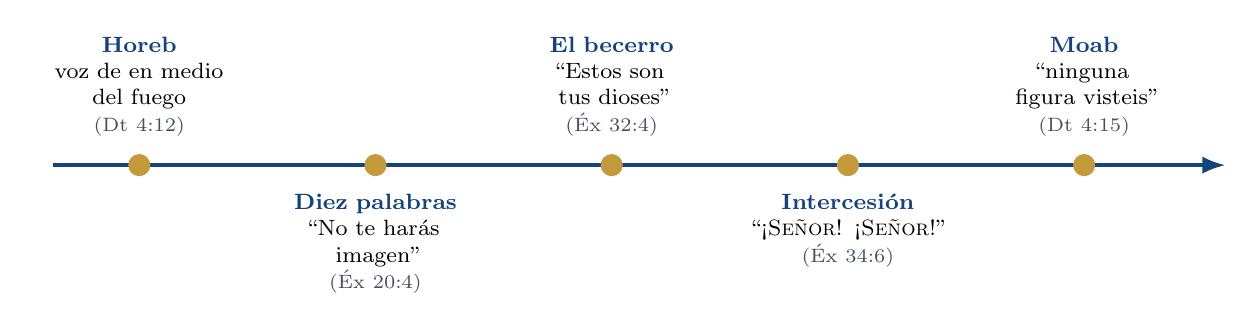
\begin{tikzpicture}[font=\footnotesize]
 \draw[line width=1.6pt,azul,-{Latex[length=3mm]}] (-0.3,0) -- (14.6,0);
 \foreach \x/\t/\b/\r/\pos in {0.8/{Horeb}/{voz de en medio del fuego}/{Dt 4:12}/above,
   3.8/{Diez palabras}/{``No te harás imagen''}/{Éx 20:4}/below,
   6.8/{El becerro}/{``Estos son tus dioses''}/{Éx 32:4}/above,
   9.8/{Intercesión}/{``¡\SENOR! ¡\SENOR!''}/{Éx 34:6}/below,
   12.8/{Moab}/{``ninguna figura visteis''}/{Dt 4:15}/above}{
  \fill[dorado] (\x,0) circle (4pt);
  \node[\pos=7pt,text width=2.6cm,align=center] at (\x,0) {\textbf{\textcolor{azul}{\t}}\\ \b\\ {\scriptsize\color{gris}(\r)}};}
\end{tikzpicture}\par
{\footnotesize\color{gris}\textit{Figura 6.} De Horeb a Moab. \textit{Nota.} Elaboración propia.}
\end{center}

La idolatría empieza por querer ver. Y Dios respondió al becerro no con una imagen, sino con su Nombre proclamado: ``¡\SENOR! ¡\SENOR! fuerte, misericordioso y piadoso'' (Éx 34:6). Incluso en el perdón se dio a conocer por la palabra.

\subsection{La lista de figuras, en Pablo}

La lista de Dt 4:16--18 reaparece, siglos después, en la carta a los Romanos, donde Pablo describe la idolatría humana con el vocabulario de la Septuaginta:

\begin{center}\small\renewcommand{\arraystretch}{1.2}
\begin{tabular}{@{}L{3.6cm}L{5.2cm}L{5.2cm}@{}}
\toprule
\textbf{Dt 4:16--18} & \textbf{LXX} & \textbf{Ro 1:23} \\ \midrule
figura, efigie & \grc{ὁμοίωμα}, \grc{εἰκών} & \grc{ἐν ὁμοιώματι εἰκόνος} \\
varón o hembra & \grc{ἀρσενικοῦ ἢ θηλυκοῦ} & \grc{φθαρτοῦ ἀνθρώπου} \\
animal de la tierra & \grc{κτήνους} & \grc{τετραπόδων} \\
ave alada & \grc{ὀρνέου πτερωτοῦ} & \grc{πετεινῶν} \\
lo que se arrastra & \grc{ἑρπετοῦ} & \grc{ἑρπετῶν} \\
\bottomrule
\end{tabular}\par
{\footnotesize\color{gris}\textit{Tabla 8.} Dt 4:16--18 y Ro 1:23. \textit{Nota.} Elaboración propia con la LXX de Rahlfs-Hanhart y NA28.}
\end{center}

\begin{cita}y cambiaron la gloria del Dios incorruptible en semejanza de imagen de hombre corruptible, de aves, de cuadrúpedos y de reptiles.\fuente{(Ro 1:23)}\end{cita}

``Cambiaron la gloria'' (\grc{ἤλλαξαν τὴν δόξαν}) es también el lenguaje del Sal 106:20 en la LXX (\grc{ἠλλάξαντο τὴν δόξαν}). Lo que Horeb prohibió, el mundo entero lo hizo.

\begin{nota}[Precisión]
El eco de Dt 4:16--18 y Sal 106:20 en Ro 1:23 es lectura de varios intérpretes (cf. Dunn, 1998); se apoya en el vocabulario común de la LXX.
\end{nota}

%===================================================================
\section{Dios es Espíritu en el judaísmo}\label{sec:judaismo-esp}

\subsection{El alma y el Santo}

El Talmud se pregunta por qué David dijo cinco veces ``Bendice, alma mía, a \SENOR'' (Sal 103--104). Rabí Yehoshúa ben Leví responde que el alma se parece al Santo, bendito sea:

\hebverso{מָה הַקָּדוֹשׁ בָּרוּךְ הוּא רוֹאֶה וְאֵינוֹ נִרְאֶה \\ אַף נְשָׁמָה רוֹאָה וְאֵינָהּ נִרְאֵית}
\begin{quote}\itshape
``Como el Santo, bendito sea, ve y no es visto, así el alma ve y no es vista''.\par\hfill{\upshape\small\bfseries\textcolor{azul}{(Talmud de Babilonia, Berajot 10a)}}
\end{quote}

\begin{center}\small\renewcommand{\arraystretch}{1.2}
\begin{tabular}{@{}L{5.6cm}L{5.6cm}@{}}
\toprule
\textbf{El Santo} & \textbf{El alma} \\ \midrule
llena todo el mundo & llena todo el cuerpo \\
ve y no es visto & ve y no es vista \\
sustenta el mundo & sustenta el cuerpo \\
es puro & es pura \\
mora en lo más íntimo & mora en lo más íntimo \\
\bottomrule
\end{tabular}\par
{\footnotesize\color{gris}\textit{Tabla 9.} Las cinco semejanzas de \emph{Berajot} 10a. \textit{Nota.} Elaboración propia a partir del Talmud (edición William Davidson, Sefaria).}
\end{center}

De ahí la conclusión del pasaje: ``Venga quien tiene estas cinco cosas y alabe al que tiene estas cinco cosas''.

\begin{nota}[Precisión]
Interpretación rabínica (Talmud de Babilonia, edición William Davidson, Sefaria); traducción propia. Es una analogía: el alma es criatura, Dios no.
\end{nota}

\subsection{Maimónides: ``no es cuerpo''}

Para Maimónides, la incorporeidad de Dios no es un detalle filosófico, sino parte de la fe misma de Israel. En su comentario a la Misná (Sanedrín 10:1) la coloca como el tercero de sus trece principios, ``la negación de la corporeidad'': Dios ``no es cuerpo ni fuerza en un cuerpo''; y la funda en Dt 4:15, \heb{כִּי לֹא רְאִיתֶם כָּל תְּמוּנָה}. En el \emph{Mishné Torá} lo formula así:

\hebverso{שֶׁאֵין הַקָּדוֹשׁ בָּרוּךְ הוּא גּוּף וּגְוִיָּה}
\begin{quote}\itshape
``El Santo, bendito sea, no es cuerpo ni figura''; y un cuerpo no puede estar en dos lugares.\par\hfill{\upshape\small\bfseries\textcolor{azul}{(Maimónides, Yesodé haTorá 1:8)}}
\end{quote}

En las leyes del arrepentimiento (Teshuvá 3:7) cuenta entre los herejes (\emph{minim}) a quien dice que hay un solo Señor, ``pero que es cuerpo y tiene figura'', y recoge la enseñanza de \emph{Jaguigá} 15a: ``arriba no hay sentarse ni estar de pie''.

La liturgia canta esta convicción cada mañana. El himno \emph{Yigdal}, compuesto sobre los trece principios, dice:

\hebverso{אֵין לוֹ דְמוּת הַגּוּף וְאֵינוֹ גוּף}
\begin{quote}\itshape
``No tiene semejanza de cuerpo, ni es cuerpo''.\par\hfill{\upshape\small\bfseries\textcolor{azul}{(\emph{Yigdal}, oración de la mañana)}}
\end{quote}

\begin{nota}[Precisión]
Lecturas judías medievales; el \emph{Yigdal} se atribuye a Daniel ben Yehudá de Roma (siglo XIV). Textos según Sefaria; traducción propia.
\end{nota}

\subsection{\emph{Rúaj} en la \emph{Guía de los perplejos}}

En la \emph{Guía} (I:40), Maimónides abre con una advertencia: \heb{רוּחַ שֵׁם מִשְׁתַּתֵּף}, ``\emph{rúaj} es un nombre equívoco'', es decir, de varios sentidos. Distingue seis:

\begin{center}\small\renewcommand{\arraystretch}{1.18}
\begin{tabular}{@{}L{0.6cm}L{5.6cm}L{8.0cm}@{}}
\toprule
& \textbf{Sentido} & \textbf{Texto que cita} \\ \midrule
1 & el aire, uno de los cuatro elementos & ``el Espíritu de Dios se movía'' (Gn 1:2) \\
2 & el viento que sopla & ``el viento oriental trajo la langosta'' (Éx 10:13) \\
3 & el espíritu vital & ``soplo que va y no vuelve'' (Sal 78:39); Gn 7:15 \\
4 & lo que queda del hombre después de la muerte & ``el espíritu vuelva a Dios que lo dio'' (Ec 12:7) \\
5 & la influencia intelectual divina sobre los profetas & ``tomaré del espíritu que está en ti'' (Nm 11:17); 2 S 23:2 \\
6 & la intención, la voluntad & ``¿Quién enseñó al Espíritu de \SENOR?'' (Is 40:13) \\
\bottomrule
\end{tabular}\par
{\footnotesize\color{gris}\textit{Tabla 10.} Los sentidos de \emph{rúaj} en Maimónides, \emph{Guía de los perplejos} I:40. \textit{Nota.} Elaboración propia a partir de la versión hebrea de Samuel ibn Tibbon (Sefaria).}
\end{center}

Todo \emph{rúaj} atribuido a Dios corresponde, para él, al sentido 5 o al 6.

\begin{nota}[Precisión]
Versión hebrea de Samuel ibn Tibbon (Sefaria); traducción propia. La lectura filosófica de Maimónides, que entiende el Espíritu como ``influencia'', no coincide con la lectura cristiana del Espíritu como persona.
\end{nota}

\subsection{Los targumes y Rashi: la gloria, la voz}

Las traducciones arameas evitan decir que alguien \emph{vio} a Dios. Donde el hebreo dice ``y vieron al Dios de Israel'' (Éx 24:10), Ónkelos traduce \heb{וַחֲזוֹ יָת יְקַר אֱלָהָא דְיִשְׂרָאֵל}, ``y vieron \emph{la gloria} del Dios de Israel''; y en Dt 4:12 lee \heb{וּדְמוּת לֵיתֵיכוֹן חָזָן אֶלָּהֵן קָלָא}, ``y semejanza no veis, sino la voz''. Es la misma convicción de Deuteronomio, trasladada al arameo.

Rashi, por su parte, explica en Gn 1:2 la imagen de la creación sin darle cuerpo a Dios: ``el trono de gloria estaba en el aire y se cernía sobre las aguas por el aliento de su boca'' (\heb{בְּרוּחַ פִּיו}), ``como paloma que se cierne sobre el nido''.

\begin{nota}[Precisión]
Interpretaciones judías antiguas y medievales (Sefaria); traducción propia.
\end{nota}

\subsection{Qumrán: espíritu y verdad}

La \emph{Regla de la Comunidad} de Qumrán (1QS) enseña que Dios puso en el hombre ``dos espíritus'', el de la verdad y el de la falsedad, hasta el tiempo de su visita (1QS III 17--19). Al final, Dios purificará al hombre con ``espíritu de santidad'' y rociará sobre él ``el espíritu de verdad como aguas de purificación'' (1QS IV 20--21). Espíritu, verdad y agua: las tres palabras de Jn 4:14, 23--24 aparecen ya juntas en un texto judío anterior al evangelio.

\begin{nota}[Precisión]
Paráfrasis según García Martínez (1992) y Vermes (2004); conviene cotejar en la Leon Levy Dead Sea Scrolls Digital Library. La relación con Juan es un paralelo de lenguaje, no una dependencia demostrada.
\end{nota}

%===================================================================
\section{Dios es Espíritu en Cristo, leído con Pablo}\label{sec:cristo-esp}

\subsection{La imagen del Dios invisible}

Israel no podía hacer una imagen de Dios porque en Horeb no vio figura alguna. Pablo, judío formado en Dt 4 y en Is 31, tampoco hace imágenes de Dios. Pero confiesa que Dios mismo tiene una imagen, y que no la hizo el hombre:

\begin{cita}El es la imagen del Dios invisible, el primogénito de toda creación.\fuente{(Col 1:15)}\end{cita}

\begin{cita}Porque en él habita corporalmente toda la plenitud de la Deidad,\fuente{(Col 2:9)}\end{cita}

\begin{filologia}[Col 1:15 y 2:9]
\begin{tabular}{@{}L{4.2cm}L{1.6cm}L{9.0cm}@{}}
\grc{εἰκὼν τοῦ θεοῦ τοῦ ἀοράτου} & \grc{εἰκών} & ``imagen del Dios invisible'': la misma palabra de Ro 1:23 (\grc{εἰκόνος}), ahora para el Hijo. \\[2pt]
\grc{κατοικεῖ} & \grc{οἰκέω} & ``habita'' de modo permanente. \\[2pt]
\grc{σωματικῶς} & \grc{σῶμα} & ``corporalmente'': la plenitud de la Deidad, que no tiene cuerpo, habita en un cuerpo. \\
\end{tabular}
\end{filologia}

La única ``imagen'' legítima de Dios es el Hijo. El Dios que es Espíritu, sin cuerpo, habita en plenitud en un \destacar{cuerpo}; y eso no niega Jn 4:24, sino que lo cumple. Dios no se hizo visible renunciando a ser Espíritu, sino uniendo a sí una humanidad verdadera.

\begin{nota}[Precisión]
La autoría paulina de Colosenses se discute; la misma idea aparece en una carta indiscutida: Cristo, ``el cual es la imagen de Dios'' (2 Co 4:4).
\end{nota}

\subsection{Deuteronomio 4 cumplido: Dios se deja ver}

\begin{cita}A Dios nadie le vio jamás; el unigénito Hijo, que está en el seno del Padre, él le ha dado a conocer.\fuente{(Jn 1:18)}\end{cita}

``Le ha dado a conocer'' traduce \grc{ἐξηγήσατο}, ``lo explicó, lo narró'': el Hijo es la exégesis del Padre. El que dijo ``no me verá hombre, y vivirá'' (Éx 33:20) se deja ver en el Hijo: ``El que me ha visto a mí, ha visto al Padre'' (Jn 14:9). Pablo lo dice en su propio lenguaje cuando afirma que Dios ``resplandeció en nuestros corazones, para iluminación del conocimiento de la gloria de Dios en la faz de Jesucristo'' (2 Co 4:6).

\begin{center}
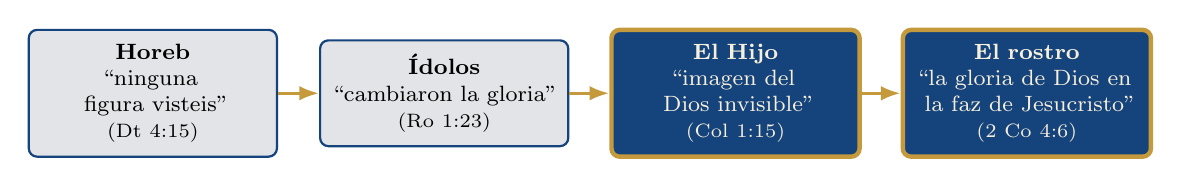
\begin{tikzpicture}[font=\footnotesize,
  caja/.style={draw=azul,line width=0.8pt,fill=gris!15,rounded corners=3pt,inner sep=5pt,align=center,text width=2.8cm},
  luz/.style={draw=dorado,line width=1.6pt,fill=azul,text=papiro,rounded corners=3pt,inner sep=5pt,align=center,text width=2.8cm}]
 \node[caja] (a) at (0,0) {\textbf{Horeb}\\ ``ninguna figura visteis''\\ {\scriptsize(Dt 4:15)}};
 \node[caja] (b) at (3.7,0) {\textbf{Ídolos}\\ ``cambiaron la gloria''\\ {\scriptsize(Ro 1:23)}};
 \node[luz] (c) at (7.4,0) {\textbf{El Hijo}\\ ``imagen del Dios invisible''\\ {\scriptsize(Col 1:15)}};
 \node[luz] (d) at (11.1,0) {\textbf{El rostro}\\ ``la gloria de Dios en la faz de Jesucristo''\\ {\scriptsize(2 Co 4:6)}};
 \draw[-{Latex[length=2.5mm]},dorado,line width=1.2pt] (a)--(b); \draw[-{Latex[length=2.5mm]},dorado,line width=1.2pt] (b)--(c); \draw[-{Latex[length=2.5mm]},dorado,line width=1.2pt] (c)--(d);
\end{tikzpicture}\par
{\footnotesize\color{gris}\textit{Figura 7.} Del Dios sin figura al rostro de Cristo. \textit{Nota.} Elaboración propia.}
\end{center}

\begin{nota}[Precisión textual]
En Jn 1:18 la NA28 lee \grc{μονογενὴς θεός}, ``el unigénito Dios''; la RVR1960 sigue el texto bizantino \grc{ὁ μονογενὴς υἱός}, ``el unigénito Hijo''.
\end{nota}

\subsection{``El Señor es el Espíritu''}

\begin{cita}Pero cuando se conviertan al Señor, el velo se quitará. Porque el Señor es el Espíritu; y donde está el Espíritu del Señor, allí hay libertad. Por tanto, nosotros todos, mirando a cara descubierta como en un espejo la gloria del Señor, somos transformados de gloria en gloria en la misma imagen, como por el Espíritu del Señor.\fuente{(2 Co 3:16--18)}\end{cita}

Pablo cita aquí Éx 34:34 casi palabra por palabra:

\begin{center}\small\renewcommand{\arraystretch}{1.22}
\begin{tabular}{@{}L{2.0cm}L{7.0cm}L{5.2cm}@{}}
\toprule
\textbf{Texto} & \textbf{Original} & \textbf{RVR1960} \\ \midrule
Éx 34:34 TM & \heb{וּבְבֹא מֹשֶׁה לִפְנֵי יְהוָה}\ldots{} \heb{יָסִיר אֶת־הַמַּסְוֶה} & ``Cuando venía Moisés delante de \SENOR\ldots{} se quitaba el velo'' \\
Éx 34:34 LXX & \grc{ἡνίκα δ’ ἂν εἰσεπορεύετο Μωυσῆς ἔναντι κυρίου\ldots{} περιῃρεῖτο τὸ κάλυμμα} & --- \\
2 Co 3:16 & \grc{ἡνίκα δὲ ἐὰν ἐπιστρέψῃ πρὸς κύριον, περιαιρεῖται τὸ κάλυμμα} & ``cuando se conviertan al Señor, el velo se quitará'' \\
2 Co 3:17 & \grc{ὁ δὲ κύριος τὸ πνεῦμά ἐστιν} & ``el Señor es el Espíritu'' \\
\bottomrule
\end{tabular}\par
{\footnotesize\color{gris}\textit{Tabla 11.} Éx 34:34 en 2 Co 3:16--17. \textit{Nota.} Elaboración propia con la BHS, la LXX y NA28.}
\end{center}

El ``Señor'' (\grc{κύριος}) ante quien Moisés se quitaba el velo es el \SENOR{} del Sinaí. Pablo explica que a ese \SENOR{} se lo encuentra hoy ``en el Espíritu'': el velo cae cuando uno se vuelve al Señor que es Espíritu. Así, el Dios que en Horeb habló sin figura es el mismo que ahora, por su Espíritu, transforma a los suyos ``en la misma imagen'', la imagen del Hijo.

\begin{nota}[Precisión]
``El Señor es el Espíritu'' no confunde al Hijo con el Espíritu: es una exégesis de Éx 34, donde ``el Señor'' del texto se refiere al Espíritu que vivifica (2 Co 3:6). Lectura sostenida por Dunn (1998) y Hays (1989).
\end{nota}

\subsection{Pablo en Atenas}

Ante los filósofos de Atenas, Pablo predica al Dios que es Espíritu con el lenguaje de Israel:

\begin{cita}El Dios que hizo el mundo y todas las cosas que en él hay, siendo Señor del cielo y de la tierra, no habita en templos hechos por manos humanas, ni es honrado por manos de hombres, como si necesitase de algo; pues él es quien da a todos vida y aliento y todas las cosas.\fuente{(Hch 17:24--25)}\end{cita}

\begin{cita}Siendo, pues, linaje de Dios, no debemos pensar que la Divinidad sea semejante a oro, o plata, o piedra, escultura de arte y de imaginación de hombres.\fuente{(Hch 17:29)}\end{cita}

Cada frase tiene su raíz en la Escritura de Israel. ``No en templos hechos de mano'' (\grc{οὐκ ἐν χειροποιήτοις ναοῖς}) recoge a Salomón (1 R 8:27) y a Isaías (66:1); ``aliento'' (\grc{πνοή}) recoge el soplo de Gn 2:7 e Is 42:5; y la prohibición de imaginar a Dios ``semejante a oro, o plata, o piedra'' es Dt 4 predicado a griegos.

\begin{nota}[Precisión]
El discurso fue transmitido por Lucas; se usa aquí como testimonio de la predicación de Pablo.
\end{nota}

\subsection{El nuevo templo: ni Gerizim ni Jerusalén}

\begin{cita}porque por medio de él los unos y los otros tenemos entrada por un mismo Espíritu al Padre\ldots{} en quien vosotros también sois juntamente edificados para morada de Dios en el Espíritu.\fuente{(Ef 2:18, 22)}\end{cita}

\begin{cita}¿No sabéis que sois templo de Dios, y que el Espíritu de Dios mora en vosotros?\fuente{(1 Co 3:16)}\end{cita}

Lo que Jesús anunció en Sicar, ``ni en este monte ni en Jerusalén'', Pablo lo ve cumplido: el templo es un pueblo, y Dios lo habita \grc{ἐν πνεύματι}, ``en el Espíritu''. Samaritanos y judíos discutían por un monte; Pablo ve a judíos y gentiles, ``los unos y los otros'', con acceso ``por un mismo Espíritu al Padre''. Es, en otras palabras, la adoración ``al Padre'' de Jn 4:21, 23.

\begin{center}
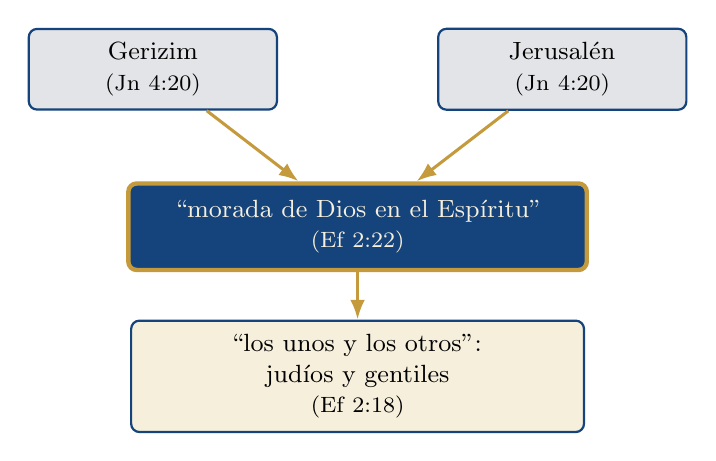
\begin{tikzpicture}[font=\small,
  caja/.style={draw=azul,line width=0.8pt,fill=papiro,rounded corners=3pt,inner sep=5pt,align=center}]
 \node[caja,text width=2.8cm,fill=gris!15] (g) at (-2.6,2.0) {Gerizim\\ {\footnotesize(Jn 4:20)}};
 \node[caja,text width=2.8cm,fill=gris!15] (j) at (2.6,2.0) {Jerusalén\\ {\footnotesize(Jn 4:20)}};
 \node[draw=dorado,line width=1.6pt,fill=azul,text=papiro,rounded corners=3pt,text width=5.4cm,align=center,inner sep=6pt] (t) at (0,0) {``morada de Dios en el Espíritu''\\ {\footnotesize(Ef 2:22)}};
 \node[caja,text width=5.4cm] (p) at (0,-1.9) {``los unos y los otros'': judíos y gentiles\\ {\footnotesize(Ef 2:18)}};
 \draw[-{Latex[length=2.5mm]},dorado,line width=1.1pt](g)--(t); \draw[-{Latex[length=2.5mm]},dorado,line width=1.1pt](j)--(t); \draw[-{Latex[length=2.5mm]},dorado,line width=1.1pt](t)--(p);
\end{tikzpicture}\par
{\footnotesize\color{gris}\textit{Figura 8.} Del monte al pueblo: la morada en el Espíritu. \textit{Nota.} Elaboración propia.}
\end{center}

\begin{nota}[Precisión]
La autoría paulina de Efesios se discute; 1 Co 3:16 dice lo mismo en una carta indiscutida.
\end{nota}

\subsection{``En espíritu servimos a Dios''}

\begin{cita}Porque nosotros somos la circuncisión, los que en espíritu servimos a Dios y nos gloriamos en Cristo Jesús, no teniendo confianza en la carne.\fuente{(Flp 3:3)}\end{cita}

\begin{cita}Así que, hermanos, os ruego por las misericordias de Dios, que presentéis vuestros cuerpos en sacrificio vivo, santo, agradable a Dios, que es vuestro culto racional.\fuente{(Ro 12:1)}\end{cita}

Pablo toma el vocabulario del culto del templo, \grc{λατρεύοντες} (Flp 3:3) y \grc{λατρεία} (Ro 12:1), y opone ``espíritu'' a ``carne'' (Flp 3:3) como lo hacía Is 31:3. Pero el culto nuevo no suprime el cuerpo: lo ofrece entero. El ``culto racional'' (\grc{λογικὴν λατρείαν}) es la adoración de Jn 4:24 vivida en lo cotidiano.

\begin{nota}[Precisión textual]
En Flp 3:3, NA28 y el texto bizantino leen \grc{πνεύματι θεοῦ λατρεύοντες}, ``los que servimos por el Espíritu de Dios''; la RVR1960 sigue la lectura ``servimos a Dios''.
\end{nota}

\subsection{``¡Abba, Padre!''}

\begin{cita}Pues no habéis recibido el espíritu de esclavitud para estar otra vez en temor, sino que habéis recibido el espíritu de adopción, por el cual clamamos: ¡Abba, Padre! El Espíritu mismo da testimonio a nuestro espíritu, de que somos hijos de Dios.\fuente{(Ro 8:15--16)}\end{cita}

Jesús habló de adorar ``al Padre'' (Jn 4:21, 23); Pablo muestra cómo ocurre: el Espíritu nos hace decir ``Abba''. \grc{αὐτὸ τὸ πνεῦμα συμμαρτυρεῖ τῷ πνεύματι ἡμῶν}: el Espíritu de Dios testifica \emph{con} nuestro espíritu. Espíritu con espíritu: esa es la comunión que Jn 4:24 pide. Y esa comunión alcanza también al cuerpo: ``si el Espíritu de aquel que levantó de los muertos a Jesús mora en vosotros, el que levantó de los muertos a Cristo Jesús vivificará también vuestros cuerpos mortales por su Espíritu que mora en vosotros'' (Ro 8:11).

\subsection{El postrer Adán, espíritu vivificante}

\begin{cita}Así también está escrito: Fue hecho el primer hombre Adán alma viviente; el postrer Adán, espíritu vivificante.\fuente{(1 Co 15:45)}\end{cita}

\begin{filologia}[1 Co 15:45 y Gn 2:7]
\begin{tabular}{@{}L{2.6cm}L{1.6cm}L{10.6cm}@{}}
Gn 2:7 LXX & --- & \grc{ἐγένετο ὁ ἄνθρωπος εἰς ψυχὴν ζῶσαν}: ``fue el hombre un alma viviente''. \\[2pt]
1 Co 15:45 & --- & \grc{ὁ ἔσχατος Ἀδὰμ εἰς πνεῦμα ζῳοποιοῦν}: ``el postrer Adán, espíritu que da vida''. \\[2pt]
\grc{πνευματικόν} & \grc{πνεῦμα} & ``espiritual'' (15:44): el cuerpo de resurrección no es inmaterial, sino animado por el Espíritu. \\
\end{tabular}
\end{filologia}

El primer Adán \destacar{recibió} aliento (Gn 2:7); el último Adán \destacar{da} vida. Cristo resucitado hace lo que solo hace el Dios que es Espíritu: vivificar (Ez 37:14; Jn 6:63).

\subsection{Síntesis paulina}

\begin{center}
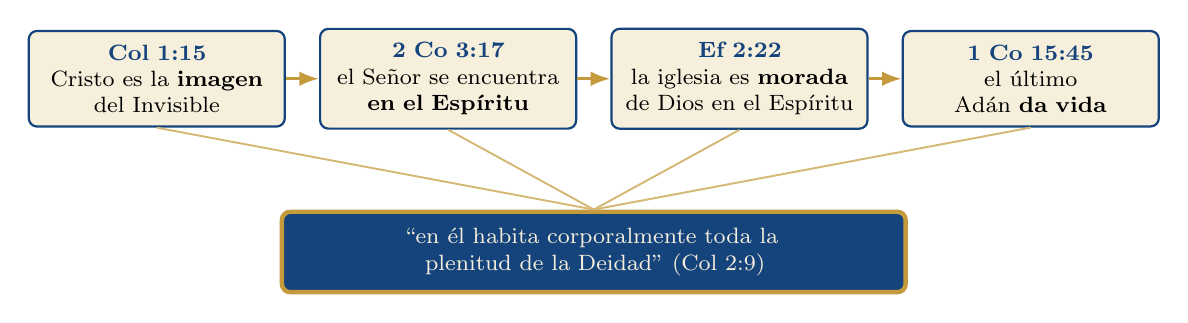
\begin{tikzpicture}[font=\footnotesize,
  caja/.style={draw=azul,line width=0.8pt,fill=papiro,rounded corners=3pt,inner sep=5pt,align=center,text width=2.9cm}]
 \node[caja] (a) at (0,0) {\textbf{\textcolor{azul}{Col 1:15}}\\ Cristo es la \textbf{imagen} del Invisible};
 \node[caja] (b) at (3.7,0) {\textbf{\textcolor{azul}{2 Co 3:17}}\\ el Señor se encuentra \textbf{en el Espíritu}};
 \node[caja] (c) at (7.4,0) {\textbf{\textcolor{azul}{Ef 2:22}}\\ la iglesia es \textbf{morada} de Dios en el Espíritu};
 \node[caja] (d) at (11.1,0) {\textbf{\textcolor{azul}{1 Co 15:45}}\\ el último Adán \textbf{da vida}};
 \draw[-{Latex[length=2.5mm]},dorado,line width=1.1pt](a)--(b); \draw[-{Latex[length=2.5mm]},dorado,line width=1.1pt](b)--(c); \draw[-{Latex[length=2.5mm]},dorado,line width=1.1pt](c)--(d);
 \node[draw=dorado,line width=1.6pt,fill=azul,text=papiro,rounded corners=3pt,text width=7.5cm,align=center,inner sep=6pt] (e) at (5.55,-2.2) {``en él habita corporalmente toda la plenitud de la Deidad'' (Col 2:9)};
 \foreach \i in {a,b,c,d}\draw[dorado!70,line width=0.7pt](\i.south)--(e.north);
\end{tikzpicture}\par
{\footnotesize\color{gris}\textit{Figura 9.} Dios es Espíritu, revelado en Cristo. \textit{Nota.} Elaboración propia.}
\end{center}

El Dios que es Espíritu se da a conocer en el Hijo y se da a sí mismo en el Espíritu. La tesis de esta obra, que la plenitud de los atributos habita en Cristo (Col 2:9), adopta aquí una forma particular: la plenitud de un Dios sin cuerpo habita ``corporalmente'' en Jesús.

%===================================================================
\section{Aplicación: adorar al Dios que es Espíritu}

Jesús no dijo ``Dios es Espíritu'' para describir a Dios en abstracto, sino para responder cómo se le adora. La aplicación, por tanto, nace del mismo texto.

\subsection{Adorar sin monte}

\begin{cita}\SENOR{} dijo así: El cielo es mi trono, y la tierra estrado de mis pies; ¿dónde está la casa que me habréis de edificar, y dónde el lugar de mi reposo?\ldots{} pero miraré a aquel que es pobre y humilde de espíritu, y que tiembla a mi palabra.\fuente{(Is 66:1--2)}\end{cita}

Los lugares sirven, pero no contienen a Dios. El \SENOR{} mira al ``humilde de espíritu'' (\heb{נְכֵה־רוּחַ}). Ningún edificio, ritual o emoción garantiza la adoración, y tampoco la impide: ``Mas tú, cuando ores, entra en tu aposento, y cerrada la puerta, ora a tu Padre que está en secreto; y tu Padre que ve en lo secreto te recompensará en público'' (Mt 6:6).

\subsection{Sin imágenes, ni de piedra ni de la mente}

\begin{cita}¿A qué, pues, haréis semejante a Dios, o qué imagen le compondréis?\fuente{(Is 40:18)}\end{cita}

``¿Qué semejanza le pondréis?'' (\heb{וּמַה־דְּמוּת תַּעַרְכוּ לוֹ}). Hoy pocos tallan ídolos, pero muchos se forman un dios a su medida: un Dios solo ``útil'', solo ``cercano'' o solo ``lejano''. A Dios lo conocemos por lo que él \emph{dice} de sí mismo (Dt 4:12) y por el Hijo (Jn 1:18), no por lo que imaginamos. ``Hijitos, guardaos de los ídolos'' (1 Jn 5:21).

\subsection{Cuatro respuestas}

\begin{enumerate}
\item \textbf{Adorar} en espíritu y en verdad, en cualquier lugar y con toda la vida: ``que presentéis vuestros cuerpos en sacrificio vivo'' (Jn 4:24; Ro 12:1).
\item \textbf{Escuchar}, porque Dios se da a conocer por su palabra y no por imágenes: en Horeb hubo ``voz de palabras'' y ninguna figura (Dt 4:12).
\item \textbf{Andar} conducidos por su Espíritu y no por la carne: ``Andad en el Espíritu, y no satisfagáis los deseos de la carne'' (Gá 5:16); ``Si vivimos por el Espíritu, andemos también por el Espíritu'' (Gá 5:25).
\item \textbf{Esperar}, porque el Espíritu que mora en nosotros ``vivificará también vuestros cuerpos mortales'' (Ro 8:11): el Dios que sopló en el polvo (Gn 2:7) y sobre los huesos secos (Ez 37:9) soplará otra vez.
\end{enumerate}

Como atributo, ser Espíritu es incomunicable: solo Dios es espíritu increado, infinito y fuente de toda vida. Pero es comunicable como reflejo, porque Dios formó el espíritu del hombre dentro de él (Zac 12:1) y por su Espíritu lo hace capaz de adorarle. Las preguntas que deja el atributo son personales:

\begin{itemize}
\item ¿Dónde está hoy nuestro ``monte'': el lugar, el estilo o la emoción sin los que creemos que no podemos adorar?
\item ¿Qué imagen de Dios nos hemos formado que no viene de su palabra?
\item ¿Nuestro culto se queda en la reunión, o llega al cuerpo y a la semana entera (Ro 12:1)?
\item ¿Vivimos como quienes tienen en sí el Espíritu del Dios vivo (Ro 8:11)?
\end{itemize}

%===================================================================
\section{Síntesis}

\begin{tcolorbox}[colback=papiro,colframe=azul,boxrule=1pt,arc=3pt]
``Dios es Espíritu'' (Jn 4:24). La palabra hebrea \emph{rúaj} une viento, aliento y espíritu: lo invisible que es real y da vida. Dios es el ``Dios de los espíritus de toda carne'' (Nm 16:22): sin cuerpo, sin figura, presente en todo lugar y fuente de toda vida. En Horeb se reveló como voz sin figura (Dt 4:12), y por eso Israel no debía hacer imágenes. En Sicar, Jesús dejó atrás la disputa de los montes: el Padre busca adoradores en espíritu y en verdad. Pablo lo ve cumplido: Cristo es ``la imagen del Dios invisible'' (Col 1:15), en él habita la plenitud ``corporalmente'' (Col 2:9), y la iglesia es ``morada de Dios en el Espíritu'' (Ef 2:22).
\end{tcolorbox}

\begin{center}\small\renewcommand{\arraystretch}{1.3}
\begin{tabular}{@{}L{3.0cm}L{11.4cm}@{}}
\toprule
\textbf{Mirada} & \textbf{Aporte al atributo} \\ \midrule
Hebrea & \emph{rúaj} (viento, aliento, espíritu); ``carne, y no espíritu'' (Is 31:3); voz sin figura (Dt 4:12); ``Dios de los espíritus de toda carne'' (Nm 16:22); los ídolos sin \emph{rúaj} (Jer 10:14). \\
Judía & El alma y el Santo (\emph{Berajot} 10a); ``no es cuerpo'' (Maimónides; \emph{Yigdal}); la Torá habla en lenguaje humano; los targumes: ``la gloria'', ``la voz''; Qumrán: espíritu de verdad y aguas. \\
Teológica & No ``un espíritu'' entre otros; incorpóreo y por eso presente en todo lugar; invisible, conocido solo por revelación (2 Co 4:6). \\
Paulina & Imagen del Invisible (Col 1:15); ``el Señor es el Espíritu'' (2 Co 3:17); templo en el Espíritu (Ef 2:22); culto racional (Ro 12:1); ``¡Abba, Padre!'' (Ro 8:15); el postrer Adán da vida (1 Co 15:45). \\
\bottomrule
\end{tabular}\end{center}

\begin{cita}Mas alábese en esto el que se hubiere de alabar: en entenderme y conocerme, que yo soy \SENOR{}, que hago misericordia, juicio y justicia en la tierra; porque estas cosas quiero, dice \SENOR{}.\fuente{(Jer 9:24 [9:23])}\end{cita}

``Entenderme y conocerme'': al Dios que es Espíritu no se le conoce mirando, sino escuchando; y, llegada la plenitud de los tiempos, mirando el rostro de Jesucristo.

%===================================================================
\section*{Compendio bíblico}
\begin{center}\small\renewcommand{\arraystretch}{1.12}
\begin{tabular}{@{}L{2.2cm}L{5.0cm}|L{2.2cm}L{5.0cm}@{}}
\toprule
Gn 1:2 & ``el Espíritu de Dios se movía'' & Jn 1:18 & ``A Dios nadie le vio jamás'' \\
Gn 2:7 & ``sopló en su nariz aliento de vida'' & Jn 3:8 & ``El viento sopla de donde quiere'' \\
Éx 33:20 & ``no me verá hombre, y vivirá'' & Jn 4:24 & ``Dios es Espíritu'' \\
Nm 16:22 & ``Dios de los espíritus de toda carne'' & Jn 6:63 & ``El espíritu es el que da vida'' \\
Nm 27:16 & ``Dios de los espíritus de toda carne'' & Jn 14:9 & ``ha visto al Padre'' \\
Dt 4:12 & ``ninguna figura visteis'' & Lc 24:39 & ``un espíritu no tiene carne ni huesos'' \\
1 R 8:27 & ``los cielos\ldots{} no te pueden contener'' & Hch 17:24--29 & ``no habita en templos'' \\
Sal 33:6 & ``por el aliento de su boca'' & Ro 1:23 & ``cambiaron la gloria'' \\
Sal 139:7 & ``¿A dónde me iré de tu Espíritu?'' & Ro 8:15--16 & ``¡Abba, Padre!'' \\
Ec 12:7 & ``el espíritu vuelva a Dios'' & Ro 12:1 & ``vuestro culto racional'' \\
Is 31:3 & ``carne, y no espíritu'' & 1 Co 2:11 & ``el Espíritu de Dios'' \\
Is 40:18 & ``¿qué imagen le compondréis?'' & 1 Co 15:45 & ``espíritu vivificante'' \\
Is 42:5 & ``espíritu a los que por ella andan'' & 2 Co 3:17 & ``el Señor es el Espíritu'' \\
Is 66:1--2 & ``humilde de espíritu'' & 2 Co 4:6 & ``en la faz de Jesucristo'' \\
Jer 10:14 & ``no hay espíritu en ella'' & Ef 2:22 & ``morada de Dios en el Espíritu'' \\
Jer 23:24 & ``¿No lleno yo\ldots{} el cielo y la tierra?'' & Col 1:15 & ``la imagen del Dios invisible'' \\
Ez 37:9, 14 & ``pondré mi Espíritu en vosotros'' & Col 2:9 & ``corporalmente'' \\
Zac 12:1 & ``forma el espíritu del hombre'' & He 12:9 & ``Padre de los espíritus'' \\
\bottomrule
\end{tabular}\par
{\footnotesize\color{gris}\textit{Tabla 12.} Compendio bíblico del atributo. \textit{Nota.} Textos de la RVR1960.}
\end{center}

%===================================================================
\section*{Glosario}
\begin{description}\setlength{\itemsep}{2pt}
\item[Antropomorfismo] Lenguaje que describe a Dios con rasgos del cuerpo humano (mano, ojos, brazo).
\item[\emph{Aóratos}] (\grc{ἀόρατος}). Invisible (Col 1:15; 1 Ti 1:17; He 11:27).
\item[\emph{Basar}] (\heb{בָּשָׂר}). Carne; lo perecedero frente al espíritu (Is 31:3).
\item[\emph{Eikón}] (\grc{εἰκών}). Imagen (Ro 1:23; 2 Co 4:4; Col 1:15).
\item[\emph{Elohé harujot}] (\heb{אֱלֹהֵי הָרוּחֹת}). ``Dios de los espíritus'' (Nm 16:22; 27:16).
\item[\emph{Exegéomai}] (\grc{ἐξηγέομαι}). Explicar, narrar, dar a conocer (Jn 1:18).
\item[Gerizim] (\heb{גְּרִזִּים}). Monte de la bendición (Dt 11:29); centro del culto samaritano.
\item[Incorporeidad] Condición de lo que no tiene cuerpo.
\item[\emph{Latreía}] (\grc{λατρεία}). Culto, servicio sagrado (Ro 12:1; Flp 3:3).
\item[\emph{Neshamá}] (\heb{נְשָׁמָה}). Aliento vital (Gn 2:7; Pr 20:27).
\item[\emph{Pneûma}] (\grc{πνεῦμα}). Viento, aliento, espíritu (Jn 3:8; 4:24).
\item[\emph{Pneumatikós}] (\grc{πνευματικός}). Espiritual (1 Co 2:15; 15:44).
\item[\emph{Proskynéō}] (\grc{προσκυνέω}). Adorar, postrarse (Jn 4:20--24).
\item[\emph{Rúaj}] (\heb{רוּחַ}). Viento, aliento, espíritu (Gn 1:2; Ez 37:9).
\item[\emph{Somatikós}] (\grc{σωματικῶς}). Corporalmente (Col 2:9).
\item[\emph{Temuná}] (\heb{תְּמוּנָה}). Figura, forma visible (Dt 4:12, 15).
\item[\emph{Tsélem}] (\heb{צֶלֶם}). Imagen (Gn 1:27).
\item[\emph{Yigdal}] (\heb{יִגְדַּל}). Himno litúrgico basado en los trece principios de Maimónides.
\end{description}

\section*{Referencias}
\refapa{Chávez, M. (1992). \emph{Diccionario de hebreo bíblico}. Editorial Mundo Hispano.}
\refapa{Dunn, J.~D.~G. (1998). \emph{The theology of Paul the apostle}. Eerdmans.}
\refapa{Elliger, K., \& Rudolph, W. (Eds.). (1997). \emph{Biblia Hebraica Stuttgartensia} (5.ª ed.). Deutsche Bibelgesellschaft.}
\refapa{García Martínez, F. (1992). \emph{Textos de Qumrán}. Trotta.}
\refapa{Gerizim, Mount. (2007). En F. Skolnik \& M. Berenbaum (Eds.), \emph{Encyclopaedia Judaica} (2.ª ed.). Macmillan Reference USA.}
\refapa{Hays, R.~B. (1989). \emph{Echoes of Scripture in the letters of Paul}. Yale University Press.}
\refapa{MacArthur, J. (2011). \emph{Biblia de estudio MacArthur} (notas). Grupo Nelson.}
\refapa{Maimónides. (s.f.). \emph{Comentario a la Misná} [Sanedrín 10:1]; \emph{Mishné Torá} [Yesodé haTorá 1:7--9; Teshuvá 3:7]. Sefaria. https://www.sefaria.org}
\refapa{Maimónides. (s.f.). \emph{Guía de los perplejos} [I:40] (S. ibn Tibbon, Trad. hebrea). Sefaria. https://www.sefaria.org}
\refapa{Nestle, E., \& Aland, K. (Eds.). (2012). \emph{Novum Testamentum Graece} (28.ª ed.). Deutsche Bibelgesellschaft.}
\refapa{Pink, A. W. (2020). \emph{Los atributos de Dios} (E. Rodríguez Cruz, Trad.). Chapel Library. (Obra original publicada en 1930)}
\refapa{Rahlfs, A., \& Hanhart, R. (Eds.). (2006). \emph{Septuaginta} (Ed. rev.). Deutsche Bibelgesellschaft.}
\refapa{Rashi. (s.f.). \emph{Comentario a la Torá} [Gn 1:2; Nm 16:22; 27:16]. Sefaria. https://www.sefaria.org}
\refapa{\emph{Santa Biblia: Reina-Valera 1960}. (1960). Sociedades Bíblicas en América Latina.}
\refapa{\emph{Sidur} [\emph{Yigdal}]. (1981). \emph{The Metsudah siddur}. Sefaria. https://www.sefaria.org}
\refapa{Steinsaltz, A. (Ed.). (2017). \emph{Koren Talmud Bavli: Edición William Davidson} [Berajot 10a]. Sefaria. https://www.sefaria.org}
\refapa{Strong, J. (1890). \emph{The exhaustive concordance of the Bible}. Hunt \& Eaton.}
\refapa{\emph{Targum Ónkelos} [Gn 1:2; Éx 24:10; Nm 16:22; Dt 4:12]; \emph{Targum Jonatán a los Profetas} [Is 31:3]. (s.f.). Sefaria. https://www.sefaria.org}
\refapa{Tov, E. (2012). \emph{Textual criticism of the Hebrew Bible} (3.ª ed.). Fortress Press.}
\refapa{Vermes, G. (2004). \emph{The complete Dead Sea Scrolls in English} (Ed. rev.). Penguin.}
\refapa{Vine, W.~E. (1999). \emph{Diccionario expositivo de palabras del Antiguo y del Nuevo Testamento exhaustivo}. Caribe.}

\end{document}
